\chapter{Contexte scientifique et problématique} % Main chapter title

\label{Perspectives} % For referencing the chapter elsewhere, use \ref{Chapter1}

Ce chapitre décrit des perspectives liées à ma recherche en cours sur l'exploration de données bioinformatique en agronomie.
Je souhaiterai présenter les directions de mes activités de recherche et leurs évolutions dans les cinq prochaines années. Toutes les perspectives présentées dans ce chapitre sont liées aux étudiants que je supervise et aux projets dans lesquels je participe.



% Ce chapitre décrit les grandes lignes des recherches menées relatives à l'exploration et l'exploitation de données bioinformatique en agronomie. Les diverses problématiques présentées sont liées aux projets dans lesquels je suis impliqué et je détaillerai pour chacune d'elles leurs acquis, évolutions et perpectives envisagées.
\section{Contexte scientifique et problématique}

Le riz est la première céréale mondiale en termes de production pour l'alimentation humaine. Cultivée dans les zones tropicales, elle pose un enjeu majeur dans les années futures. Pour relever les défis de la croissance alimentaire mondiale dans un contexte de changement climatique, il est crucial d'améliorer les capacités de production notamment par l’amélioration génétiques des plantes. \\

\subsection{Le séquençage des génomes de riz}
Le dogme central de la biologie moléculaire\label{dogma} suggère que tous les processus biologiques d'un organisme proviennent des informations codées dans son ADN génomique. De fait, décrypter de la séquence complète du génome (i.e. la totalité de l'ADN repartie sur les chromosomes) permettrait de comprendre de l'ensemble des mécanismes biologiques.\\

\begin{figure}[!ht]
    \centering
    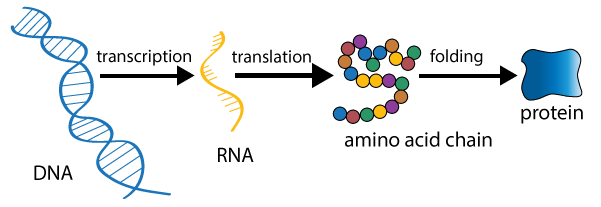
\includegraphics[width=0.90\textwidth]{hdr_manuscript/Figures/central-dogma.png}
    \caption{Le dogme central de la biologie moléculaire indique que l'information contenue dans l'ADN génomique est successivement transformé en ARN, chaîne amino acides et protéine. Crédits:biosocialmethods.isr.umich.edu}
    \label{fig:dogma}
\end{figure}



Cette hypothèse, a entraîné dés 1990, le développement de grands projets dont le projet international de séquençage du génome du riz (IRGSP) en 1998, regroupant des chercheurs de dix pays, dont des chercheurs du Français. Le riz, particulièrement l'espèce Oryza sativa qui est la plus représentative du genre, fut le premier projet de séquençage pour les plantes cultivée. Oryza sativa est un genome diploide de type AA qui comprend deux sous-espèces principales\ref{genus}: la variété japonica à grain court et collant, et la variété de riz indica à grain long et non collante. Les variétés Japonica sont généralement cultivées dans le nord-est de l'Asie et dans les zones montagneuses tandis que les variétés Indica sont principalement des riz de plaine, cultivés principalement en immersion, dans les zone tropicale en Asie. Japonica (variété nipponbare) fut le premier génome être séquencé. Une séquence représentant une couverture de 95\% de sa longueur totale de 389 Mega-bases fut achevée en 2004. La séquence génomique de haute qualité servit pendant de nombreuses années de modèle aux projets de séquençage du génome d'autres cultures céréalières possédant de grands génomes et des contenus chromosomique complexes \cite{matsumoto_nipponbare_2016}. La recherche de gènes  \textit{ab initio} (i.e. localiser la position des gènes sur le génome) prédit un total de 37 544 séquences codant pour des protéines et une comparaison avec le génome d'Arabidopsis thaliana révéla que 2 859 gènes de riz n'ont pas été observés auparavant dans cette espèce voisine. Indica fut séquencé presque simultanément mais avec une qualité bien inférieure.\\

L'annotation du génome (i.e. assigner une fonction aux gènes) est absolument essentielle pour utiliser les informations sur le génome dans les études biologiques. Dans le cas du riz, deux projets concurrents ont produit une annotation différente. La première fut réalisé par le TIGR (The institute of Genome Research) et aujourd'hui gérée par la Michigan State University (MSU)\footnote{\url{http://rice.plantbiology.msu.edu/cgi-bin/gbrowse/rice/}}. Alors que les membres de l'IRGSP ont lancé le projet officiel d'annotation du génome (RAP) publiant les données à partir de RAP-DB\footnote{\url{http://rapdb.dna. affrc.go.jp}}. Dés lors, les deux systèmes ont co-existé encore aujourd'hui avec un recouvrement partiel des annotations, ce qui complique la tache des scientifiques pour l'analyse de leur données.\\

Dans les années qui ont suivies, de nombreuses études de génomique fonctionnelles ont été conduites afin de mieux caractériser la fonction de ces gènes identifiés. Nombreuses de ces études consistaient à disputer les gènes par ciblages spécifiques (cf.Transgénèse\footnote{\url{https://fr.wikipedia.org/wiki/Transg\%C3\%A9n\%C3\%A8se}}) telles que celle décrites dans la section \ref{these} dans laquelle j'ai participé. A l'issue des ces premières découvertes, les scientifiques ont constaté que l'identification des gènes dans le génome ne suffit pas à expliquer les caractères phénotypiques observés chez la plante.  Par ailleurs, les analyses de diversité génétiques réalisées sur des populations de plantes de l'espèce O. sativa, révèlent des différences dans l'expression de gènes et dans la présence-absence de certains d'entre eux. Ainsi, succédant a ces premiers projets de séquençage, le projet OMAP “Oryza Map Alignment Project” fut établit dans le courant des année 2000 avec pour objectif de séquencer et étudier la structure évolutive des génomes diploïdes du groupe AA et BB (Wing et al. 2005).\\ 

\begin{figure}[!ht]
    \centering
    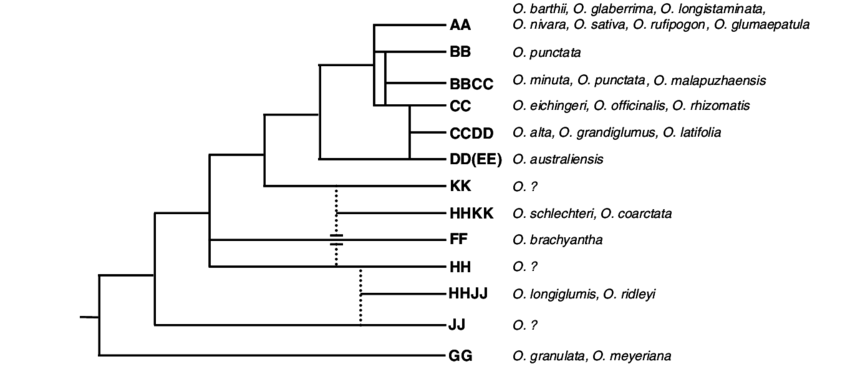
\includegraphics[width=0.9\textwidth]{hdr_manuscript/Figures/pylogenetic-tree.png}
    \caption{Arbre Phylogénétique du genre Oryza (Modifié à partir de Ge et al. 1999).  Crédits:Projet OMAP}
    \label{fig:genus}
\end{figure}

\subsection{La révolution des technologies haut-débits}
Récemment, les progrès des technologies de séquençage et des méthodes de phénotypage à haut débit conduisent à une explosion de données. Elles sont utilisées par les scientifiques pour déchiffrer la complexité du système biologique et comprendre les bases moléculaires des phénotypes et des maladies offrant une occasion unique d’accélérer l’amélioration de cette plante. Le projet de séquençage à grande échelle le plus récent pour O. sativa est le 3000 Rice Genomes Project \cite{3KRG_2018}. Ce projet, a utilisé une collection de base de 3 000 accessions de ressources génétiques de riz, sélectionnées parmi des ressources de l'Institut international de recherche sur le riz (IRRI) et de l'académie chinoise des sciences agricoles (CAAS), et comprenant des accessions provenant de 89 pays répartis en Asie du Sud-Est (33,9\%), en Asie du Sud (25,6\%) et en Chine (17,6\%) incluant des cultivars japonica et indica. Chaque génome des 3 000 accessions contenait des séquences avec une couverture de 14X en moyenne (1x correspondant a une fois le génome), ce qui indique que cette masse de données fournissait une profondeur suffisante pour la détection polymorphismes mono-nucléotidiques (SNP) fiables. Au total 17 To de données ont été obtenues. D'après une comparaison avec le génome de référence de l'IRGSP-1.0, environ 18,9 M de SNP ont été identifiés. Ces données serviront de ressource fondamentale pour la découverte de nouveaux allèles (i.e. variation d'un gène chez un individu) pour d'importants caractères utiles à l'amélioration du riz et à son adaptation au changement climatique. \\ 

Ces recherches visent principalement à comprendre la relation entre génotype et phénotype sur la base d'études d'association pan-génomique (GWAS) et fournissent des informations telles que des polymorphismes génétiques spécifiques pour une variété, la diversité génétique intra et inter population, et des informations sur l'histoire la domestication du riz en Asie.

Les études GWAS ou Genome Wide Association Studies sont des analyses biologiques étudiant les variations génétiques à l'échelle du génome pour un ensemble d'individu et pour un caractère phénotypique donnée (trait). Les marqueurs polymorphes les plus couramment utilisés pour GWAS sont les polymorphismes de séquence tels que les SNP et les variants structuraux tels que les indels (i.e. insertion ou délétion de nucléotide chez un individu par rapport au génome de référence) et les CNV (i.e. Copy Number Variation, éléments de structures répétées). Les GWAS sont maintenant préférées aux études de génétique d'association traditionnelles telles que les QTL (Quantitative Trait Loci) qui utilisent la cartographie par intervalles pour estimer la position sur la carte et l'effet de chaque QTL. Comme l'illustre la figure \ref{plot}, les locus GWAS regroupent souvent plusieurs centaines de gènes qu'il faut analyser pour identifier seulement une fraction de gènes associés au caractère (trait) étudié.  À un certain stade, chaque scientifique doit choisir les gènes à étudier expérimentalement en laboratoire. Souvent, ce choix est subjectif, car il est basé sur des connaissances partielles des interactions entre le génotype et le phénotype.


\begin{figure}[!ht]
    \centering
    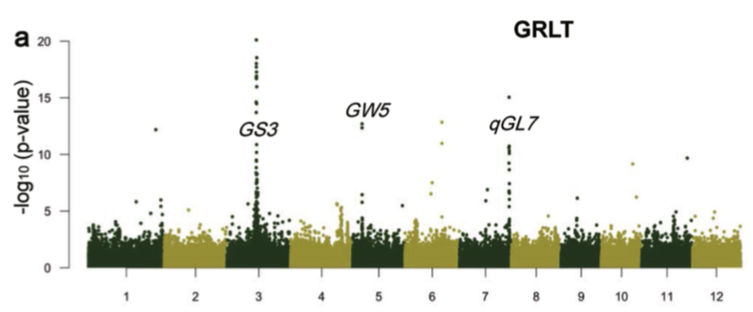
\includegraphics[width=0.8\textwidth]{hdr_manuscript/Figures/Manathan_Plot_rice.png}
    \caption{Analyse GWAS réalisée pour la longueur du grain (GRLT) chez Oryza sativa (Modifié à partir de Wang et al. 2018). Illustration d'un manathan plot montrant la corrélation entre des variants et le caractère de longueur du grain. Ici chaque point représente un SNP avec sur l'axe des abscisses sa position chromosomique et sur l'axe Y sont degré d'association. Sur cet exemple, les gènes connus ont été indiqués sur les positions et d'autres positions sont potentiellement candidates }
    \label{fig:plot}
\end{figure}

\subsection{Caractérisation des relations génotype-phénotype}
 La compréhension des relations génotype-phénotype est un des axes les plus important de la recherche tant en santé humaine avec des applications sur la prédiction des risques ou le traitement thérapeutique que pour les animaux et les plantes pour accélérer la reproduction des caractères important pour la production agricole. Or les interactions génotype-phénotype complexes à identifier. Au cours des dernières années, une multitude d'études GWAS ont identifié de nombreux variants génétiques associés à des maladies complexes ou à d'autres caractères phénotypique. Toutefois, même si ces découvertes enrichissent grandement nos connaissances sur les bases génétiques de la variation phénotypique, la plupart des variantes identifiées jusqu’à présent n’expliquent qu'une faible proportion des facteurs génétiques causaux, laissant à découvrir et expliquer l'héritabilité restante \cite{manolio2009}. Par ailleurs, même avec une compréhension complète de la génétique d'un trait phénotypique complexe, il reste difficile de prédire avec précision les variations phénotypiques à partir des codes génétiques seuls. Une des raisons et que la majorité de ces variations génétiques liées à une maladie ou à un trait se trouvent dans des régions non codantes du génomes, ce qui complique leur annotation fonctionnelle et représente le plus grand défi de l’ère «post-GWAS» \cite{freedman2011,Hou2013a}.
 Lier à l'échelle du génomes les variants génétiques à la diversité phénotypique est l’un des objectifs majeur de la biologie. Or, notre compréhension d'une telle carte génotype – phénotype ne peut être établie sans données phénotypiques détaillées \cite{houle2010}. Cependant, notre capacité à caractériser les phénomes - l'ensemble des phénotypes d'un individu - est largement en retard sur notre capacité à caractériser les génomes. En conséquence, la phénomique (i.e. phénotypage à haut débit et multi-échelle) émergea comme une discipline combinant de nouvelles technologies d'observation du vivant (i.e. caméra, capteurs, etc.) permettant d’accélérer les progrès dans notre compréhension de la relation entre génotype et phénotype.
 Les relations génotype-phénotype sont aussi très liées/sensibles aux facteurs environnementaux (e.g. la cigarette augmente fortement les risques de cancers, la sécheresse favorisera une baisse de production). Ces relations sont souvent conceptualisées \\ 

 \textit{Génotype (G) + Environnement (E) +  génotype x environnement (GxE) -> Phénotype (P)}\\
 Ainsi, pour étudier ces interactions de manière reproductible, il est nécessaire de travailler dans des conditions environnementales stables et contrôlées. 
 \\
 
\begin{figure}[!ht]
    \centering
    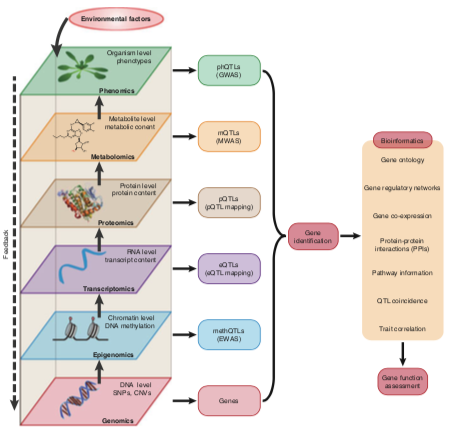
\includegraphics[width=0.9\textwidth]{hdr_manuscript/Figures/Geno-pheno.png}
    \caption{ref\cite{ChenCAK14}}
    \label{fig:geno-pheno}
\end{figure}

\subsection{Les mécanismes qui régulent l'expression des gènes}
La génomique ainsi que d'autres technologies d'analyse moléculaires haut débit comme l'épigénomique, la transcriptomique, la protéomique et la métabolomique sont devenues les méthodes d'analyses standards dans ce domaine (que l'on nomme "omique") et dont l'objectif est d'étudier le système biologique moléculaire entier. Par ailleurs, la phénomique développe des méthodes pour étudier les phénotypes de manière précise et en quantité importante. Comme le montre la figure \ref{fig:geno-pheno}, la régulation de l'expression des gènes conduisant à un phénotype peut intervenir à différents niveaux au sein d'une cellule et de l'organisme. \\
\begin{itemize}
    \item D'abords, au niveau de \textbf{l'ADN génomique}, sur lequel de simple mutations (SNP) ou des grandes modifications de sa structure (délétions, modification ou insertion de grand fragments appelés CNV) peuvent modifier l'expression des gènes.\\
    
    \item  Au niveau de \textbf{l'épigénome} - ensemble des propriétés physico- chimique de l'ADN et des protéines histones sur lesquelles il est enroulé - qui contrôle la structure de la chromatine ( complexe ADN-histones structurant un chromosome) et que des facteurs épigénétiques permettent de modifier. L'épigénomique est la discipline qui étudie l'ensemble de ses facteurs et leur lien avec la structure de la chromatine. L'épigénome est très sensible aux facteurs environnementaux externes qui agissent comme stimuli (positif ou négatif). Comme le montre la figure \ref{fig:epigenet}, des modifications chimique de la chromatine permettent de libérer l'accès a l'ADN et favoriser l'expression des gènes.
    
    \begin{figure}[!ht]
    \centering
    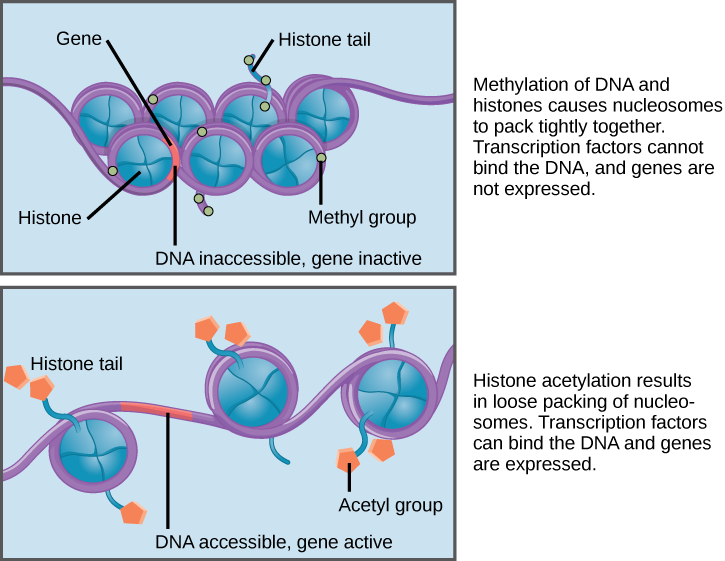
\includegraphics[width=0.8\textwidth]{hdr_manuscript/Figures/epigenet.png}
    \caption{Mécanisme d'ouverture du nucléosome - complexe histones-ADN - pour permettre la transcription des gènes. Crédits:Lumen\footnote{\url{https://courses.lumenlearning.com/wm-biology1/chapter/reading-eukaryotic-epigenetic-gene-regulation/}}}
    \label{fig:epigenet}
\end{figure}

    \item \textbf{La transcriptomique} fait référence à l'analyse de l'ensemble des molécules d'ARN, de l'ARN codant pour les protéines à l'ARN non codant. Le transcriptome peut s’appliquer à un organisme entier ou à un type de cellule spécifique. Des méthodes actuelles permettant d'identifier de manière exhaustive et ciblée l'expression de presque toutes les espèces d'ARN. L'analyse du transcriptome renseigne directement sur le taux et la dynamique (quantité et variation temporelle) d'expression des gènes, leur co-expression et leur spécificité lié a un type cellulaire ou un tissu. Il permet également des révéler des mécanismes de régulation impliquant les ARN non codant tels que les miRNA, siRNA et leurs familles.  \\
    
    \item \textbf{La protéomique} est l'étude de l'ensemble des protéines exprimées par un génome, cellule, tissu ou organisme pour un temps donné. Comme pour l'ARN, elles ont un lien direct avec les gènes à partir duquel elles sont traduites. L'action du protéome sur la régulation des gènes est multiple. Les protéines peuvent interagir directement i)  sur les gènes pour modifier leur expression (stimuler ou stopper), ii) sur les ARN pour modifier leur expression ou leur stabilité, iii) sur les protéines elles-même en auto-régulation ou interaction, iv) sur le métabolome dont elles sont les acteurs principaux. Les protéines agissent à différents niveaux dans l'organisme et sont impliqués dans tout les processus biologiques.  \\
    
    \item \textbf{La métabolomique} est l'analyse des petites molécules chimiques présent dans une cellule, tissu ou organisme. Ces molécules interviennent dans les processus biologiques comme co-facteurs catalytiques. Les réseaux (voies) métaboliques sont des séquences de réactions biochimiques impliquant les protéines et ces petites molécules. Ces réseaux peuvent être différents selon l'organisme, les stades de développement, les localisations sub-cellulaires, etc. L'information acquises sur ces réseaux constituent une base importante pour la compréhension de la biologies des systèmes.
    \item \textbf{Le phénome} représente l'ensemble des caractères phénotypiques (traits) observés chez un organisme. Selon certain expert, il peut inclure les dimensions citées précédemment, toutefois en général le phénome fait référence aux observations externes réalisées au niveau de l'individu ( e.g. la plante). Outre les traits qui sont principalement déterminés génétiquement (par exemple la couleur des cheveux), de nombreux traits dépendent d'effets environnementaux, tels que les stress biotiques ou abiotiques.\\
\end{itemize}


 
Même si les technologies permettent d'aller toujours plus loin dans l'obtention de nouvelles données, notre connaissance du système reste encore parcellaires pour élucider les mécanismes moléculaire qui régissent l'expression des caractères complexes. Les nouveaux défis consistent à comprendre les relations complexes existant entre le génome, l'épigénome, l'environnement et le phénome. Cet objectif ne peut être atteint qu'en intégrant des informations de différents niveaux dans un modèle intégrateur utilisant une approche systémique afin de comprendre le fonctionnement réel d'un système biologique et permettre de prédire les phénotypes. 

\subsection{L'intégration de données en biologie}
\subsubsection{L'hétérogénéité des systèmes}
Une meilleure compréhension des relations génotype-phénotype nécessite une intégration de données biologiques de diverse nature. Or, une caractéristique de la biologie moléculaire est que le volume et la variété des données produites par les technologies haut-débit ont une croissance exponentielle. Les bases de données constituent une source majeure de connaissances pour la recherche en sciences de la vie. Actuellement, il existe plus de 2 000 systèmes de bases de données et d'information disponibles via Internet, qui représentent ces données moléculaires \cite{NAR2019}. Chaque année, de nouvelles bases de données moléculaires et systèmes d’information utilisables via Internet apparaissent. Une caractéristique de tous ces systèmes, est que leur mises à jour tant sur les données que sur le système sont constantes. Toutefois, de dérogeant pas aux règles de financement des projets de recherches académiques qui sont en moyenne de 3 à 5 ans, on constate que la plupart de ces systèmes ont une durée de vie courte. En effet, même s'ils sont toujours disponibles sur Internet des années plus tard, leur mises à jour ou évolution est souvent stoppée. La seule chance de survie d’un nouveau système est de trouver de nouveaux financements, d'avoir un modèle économique incluant des services payants ou de créer une entreprise. Deux importantes ressources Tair et Uniprot dans le domaine ont expérimenté plusieurs modèles de financement un bilan de leur modèle pour financer leur fonctionnement et en font un bilan \cite{TAIR_sustainable_2016,Uniprot_funding_2017}. Mise à part quelques exemples comme ceux-ci, la situation reste compliquée dans la plus part des cas.  À ce stade, il est important de noter que la qualité des données présentées par ces systèmes via Internet doit être garantie par chaque fournisseur de données ou du système d’information. Jusqu'à présent, aucune norme de qualité n'a été définie pour la mise en oeuvre de ces données. La provenance des données est un élément important à prendre en compte dans les analyses réalisée à partir de données issues de plusieurs ressources distribuées\cite{ICDE2011}.\\

 Au-delà de la discussion sur la qualité des données, il est également important de mentionner que ces systèmes sont extrêmement hétérogènes.
 Dans leur article de synthèse Leser et Naumann énumèrent les formes d'hétérogénéité rencontrées que nous avons adapté \cite{dils2006}:\\
 
 \begin{itemize}
     \item  \textbf{L'hétérogénéité syntaxique} se retrouve dans le modelé de données (XML, relationnel, objet, graphe, etc.), dans les langages d’interrogation (XQuery, SQL,  OQL, SPARQL, etc.), dans les protocoles d’accès (HTTP, etc.), dans les interfaces (REST, SPOAP, .NET, etc.).
      
     \item  \textbf{L'hétérogénéité structurelle} correspond aux différences dans la représentation des données. L'autonomie de conception provoque souvent une hétérogénéité structurelle, schématique et sémantique dans l'intégration des données.  L'hétérogénéité structurelle est un cas particulier d'hétérogénéité sémantique, où différents concepts d'un modèle de données décrivent le même problème ou les mêmes données. Ils surviennent quand les schémas de deux sources décrivent différemment un même concept. Par exemple, le nom d’un employé peut être représenté par deux champs “prénom” et“nom” dans une source et par un seul champ “identité” dans une autre source. Nous pouvons également citer l’exemple d’un concept défini comme une classe dans une source de données et comme attribut dans une autre. 

     \item  \textbf{L'hétérogénéité sémantique} caractérise les différences de sens, d'interprétation, de types de termes et de concepts. Les synonymes et les homonymes jouent un rôle majeur dans ces conflits. Les synonymes sont deux  mots distincts ayant le même sens. C’est l’exemple de “publication” et  “article” qui capturent la  même information sur les articles de recherche publiés. Les homonymes sont des mots partageant la même graphie et la même prononciation mais n’ayant pas le même sens. Par   exemple,  une étoile représentant une planète et l'actrice de cinéma. \\

 \end{itemize}
 
 
Également, l'une des classifications les plus complètes provient de Pluempitiwiriyawej et Hammer, "Classification Scheme for Semantic and Schematic Heterogeneities in XML Data Sources"\cite{bergman2006}\\
 

Les différents points abordés précédemment sont la principale raison pour laquelle le processus automatique d’accès aux données reste difficile même si les données sont disponibles sur Internet. Pour les biologistes, l'inspection manuelle de ces ressources disponibles sur internet est une tâche fastidieuse pour laquelle des méthodes informatiques doivent être appliquées. Il n’est pas facile d’interroger ces données et d’avoir une réponse claire tant la masse d’information est difficile à gérer. Aujourd'hui encore le développement d'outils permettant un accès à ces données moléculaires distribuées et hétérogènes constitue une partie importante de la recherche en bioinformatique. 

\subsubsection{L'évolution des approches d'intégration de données}
Les défis majeurs actuels sont liés au développement de méthodes pour l’intégration de ces données hétérogènes et à l’enrichissement de connaissances biologiques.\\
La figure \ref{fig:databases} montre que les évolutions des méthodes d'observation du vivant ont bénéficié des avancées technologiques en informatique pour extraire de la connaissances dans les données\cite{valencia2002}.

 \begin{figure}[!ht]
    \centering
    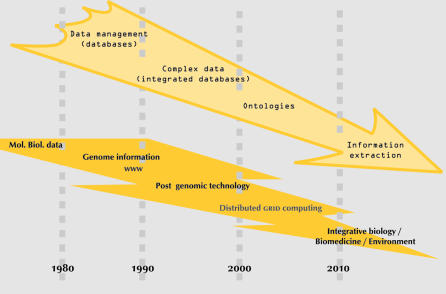
\includegraphics[width=0.8\textwidth]{hdr_manuscript/Figures/valencia2002.jpg}
    \caption{ Évolution des systèmes d'information en parallèle des méthodes biologiques. Crédits: Valencia 2002 \cite{valencia2002}}
    \label{fig:databases}
\end{figure}
Le développement de système d'intégration peut devenir extrêmement complexe si le nombre de sources à intégrer est important. En général, les systèmes d’intégration fournissent une vue unifiée de plusieurs sources hétérogènes, autonomes et répartis, facilitant ainsi l’accès à l’information. La méthode est réalisé par l’utilisation d’un schéma global ou d’une ontologie globale, qui fournit une vue réconciliée (consensuelle) des sources locales. Il existe deux   approches   pour   l’intégration :   l’intégration   matérialisée   et   l’intégration   virtuelle. \\

La première approche stocke l'ensemble des données intégrées dans un SGBB en dupliquant ces dernières à partir des sources. Cette approche nécessite de mettre à jour régulièrement les sources et réaliser des extensions du modèle global pour l'ajout de nouvelles sources. \textit{L'intégration matérialisée} présente l'avantage d'avoir des temps d'accès très rapide, car il n'y a pas de communication entre différentes sources de données, ni de limitation des requêtes. En revanche, elle nécessite un stockage volumineux et fiable. Par ailleurs, une étape importante de pré-traitement des données est nécessaire. Le processus d'ETL (Extraction Transform and Load) est la méthode désignée pour intégrer les données dans un SGBD. Elle peut s'avérer très complexe. \textit{L'intégration virtuelle} ne stocke pas les données de manière persistante en s'inspirant du modèle la médiation proposé par Wierderhold  \cite{Wiederhold1995,wiederhold1997}. Généralement, les données sont situées sur différents systèmes réparties et interrogées à l'aide d'un schéma global. Un processus d'ETL n'est pas nécessaire, contrairement à l'intégration matérialisée. Les requêtes sont gérées à partir d'un schéma global, tandis que les données sous-jacentes sont «virtuellement» disponibles. La tâche principale au système et d'offrir un protocole d’accès et un langage de requêtes commun à toutes ces sources. Par ailleurs, il doit générer des requêtes complexes pour obtenir, transformer et agréger des données adéquates provenant de différentes sources de données. La communication avec les sources fonctionne généralement a l'aide d'adaptateurs. Leurs rôles est d'adapter la requête du médiateur exprimée dans le langage commun au langage de la source, tout en utilisant le bon protocole d’accès. Étant donné que la requête utilisateur est exprimée en fonction du schéma global, une correspondance (ou mapping) entre ce schéma global et les schémas locaux (des sources) est nécessaire  afin que les requêtes puissent exécutée parles sources locales.  Ce mapping constitue un traitement clé dans le processus général. Il sera utilisé pour réécrire la requête initialement exprimée en fonction du schéma global, en des sous-requêtes exprimées, chacune, en fonction des sources locales.\\

Deux approches existent pour définir le mapping entre le schéma global et les schémas des sources: Local As View (LAV) et Global As View (GAV) \cite{Halevy2001}. Dans l’approche GAV, le schéma global est exprimé à l’aide de vues sur les schémas locaux, à l’inverse de l’approche LAV qui nécessite la description des sources locales en fonction du schéma global. Les approches LAV et GAV ont chacune des avantages et des inconvénients. Ainsi, la  LAV   favorise l’extensibilité   du   système   d’intégration   puisque   l’ajout   ou   la   suppression   des   sources   est   simple,   chaque source   étant   décrite   indépendamment   des   autres.   Mais,  la   réécriture   dans   ce   cas   est   un   problème complexe.   Quant   à   l’approche   GAV,   elle   favorise,   la   performance   du   système   quand   l’utilisateur   pose fréquemment   des   requêtes   complexes   puisque   les   algorithmes   de   réécriture   de   requêtes   sont   plus   simples. Cependant, l’ajout ou la suppression d’une source de données nécessite la mise à jour du schéma global pour l’adapter au nouvel état du système. En plus de la LAV et de la GAV, il faut mentionner l’approche GLAV qui est une combinaison des deux approches \cite{lenzerini2002}.\\


Une synthèse des principales approches d'intégration en bioinformatique réalisées au cours des dernières années ont été discutées dans Cohen-Boulakia et Leser \cite{cohen2010}. Nous en proposons ici une version modifiée et étendue:
\begin{itemize}
 
 \item \textbf{Les Systèmes de navigation hyper-texte} sont les première génération de systèmes d'intégration (1985-1995). Ils utilisent comme index, les identifiants d'entités biologiques enregistrés dans les fichiers plats aux formats spécifiques ainsi que des des liens hyper-texte faisant office de cross-références vers d'autres sources similaires. Surtout un des avantages est qu'ils utilisent des interfaces HTML permettant la recherche et la navigation (SRS \cite{srs}, Entrez \cite{entrez}). 
 \item \textbf{Les systèmes multi-bases de données} n'ont pas de schéma global. Ces systèmes génèrent de manière interactive des requêtes pour plusieurs bases de données simultanément. 
 \item \textbf{Les systèmes de base de données fédérés et les systèmes basés sur médiateur} sont des systèmes d'intégration virtuels. Ils ne stockent aucune donnée dans un schéma global. Les systèmes fédérés intègrent plusieurs systèmes de bases de données autonomes dans une base de données fédérée virtuelle unique. En règle générale, chaque base de données est inter-connectée via un réseau informatique ou, dans certains cas, le Web. Par conséquent, les bases de données peuvent être décentralisées géographiquement (K2/Kleisli \cite{k2kleisli}, DiscoveryLink \cite{discoverylink}).
 \item \textbf{Les entrepôts de données} sont des approches d'intégration matérialisées. Ils stockent les données persistantes dans un référentiel de données global, qui est généralement un SGBD relationnel (GUS \cite{k2kleisli}, Atlas \cite{atlas}, BioWarehouse \cite{biowarehouse}, Columba \cite{columba}).
\item \textbf{Les boîtes à outils} qui facilitent la construction de tels entrepôts de données sont trés populaires. Parmi elles, BioDWH \cite{biodwh} GMOD-CHADO \cite{chado_2006}, BioMART \cite{biomart2009}, intermine \cite{intermine_2012}, Tripal \cite{tripal_2011,tripal_2013,tripal_2018}.
 \item \textbf{Les systèmes utilisant des ontologies} pour l'intégration et les requêtes. (TAMBIS (Transparent Access to Multiple Bioinformatics Information Sources) \cite{tambis} et ONDEX \cite{ondex_2006,ondex_2011,Taubert2014}).
 \item \textbf{Systèmes hybrides} s'appuyant sur plusieurs technologies. Par exemple, Biozon \cite{biozon2006} combine une approche SGBD relationnelle et une représentation sous forme de graphe.\\
  
\end{itemize}

Toutes ces approches ont le même objectif: fournir des techniques pour surmonter plusieurs types de données hétérogènes et fournir un système de recherche aux scientifiques pour appuyer leurs activités de recherche et leurs expériences.
Pendant des décennies, les SGBD relationnels ont été majoritairement utilisés pour traiter des données structurées. Cependant, en raison du volume, de la rapidité d'évolution et de la variété des données, ces derniers ne peuvent souvent pas offrir les performances et le temps de latence requis pour gérer des données volumineuses et complexes. L'augmentation de la production de données non structurées issues de capteurs ou technologies haut-débit, pas seulement en biologie, fait émerger de nouveaux besoins en termes de gestion. La représentation de données massives et complexes est un champ de recherche très actif en informatique. Ainsi, de nouvelles technologies ont émergées, capables de traiter une grande variété de données et d’exécuter des applications à grande échelle sur des systèmes parallélisés, pouvant potentiellement impliquer des milliers de téraoctets de données. Elles sont regroupées sous les termes de NoSQL et NewSQL~\cite{Gajendran2012, Grolinger2013,MoniruzzamanH13}.\\

Récemment les développements de nouvelles générations de base de données NoSQL, ont ouverts de nouvelles perspectives notamment en bioinformatique. D'abords, des applications dans le domaine génomique ont été développé avec CouchDB \cite{Manyam2012,Aniceto2015}, Cassandra \cite{Gabetta2015} et MongoDB \cite{Sempere2016}. Puis les applications ont été élargies vers d'autres domaines comme la santé, le phénotype. Une étude comparative a également été faite dans le domaine de la sélection génomique et le breeding en agronomie \cite{benchmarking2019}. Par ailleurs, le développement de framework d'analyse de données volumineuse en parallèle telle que Hadoop ou Spark, a donnée lieu à des applications \cite{Schumacher2014,Nordberg2013,Taylor2010}.\\

 Concernant le développement de systèmes d'integration, de nombreuses études ont montré que la représentation d’information sous forme de graphe était mieux adaptée pour gérer l’information biologique~\cite{Have2013,Lysenko2016}.  au vu du nombre croissant de base de données de graphes se développer sur ce modèle~\cite{Hassani-Pak2016,Pareja-tobes2015}. Toutefois, ces applications utilisent une approche centralisée et fermée (i.e. les données ne sont pas facilement accessibles), à l’opposé des courants actuels qui encouragent l’open data (FAIR Data principles~\cite{Wilkinson2016a}) et l’interopérabilité des données~\cite{DzaleYeumo2017,Leonelli2017}. Elixir-Europe est une structure européenne impliquant les principaux instituts publics nationaux qui favorise le développement de services en Bioinfomatique et favorise la dissémination de l’information. Dans le domaine agronomique, des groupes de travail (RDA , DivSeek et PhenoHarmonIS) ont pour objectifs de promouvoir les bonnes pratiques de gestion et les standards d’échange de données.\\

La technologie Web Sémantique (SW) proposée par Tim Berners-Lee~\cite{berners2001semweb} offre une solution pour faciliter cette intégration et permettre l'interopérabilité entre les machines. \\

Au cours des dernières années, de nombreuses initiatives ont émergé dans la communauté biomédicale afin de fournir des environnements intégrés permettant de formuler des hypothèses scientifiques sur le rôles des gènes dans l’expression des phénotypes ou l’émergence de maladies. Parmi elles citons BIO2RDF~\cite{Belleau2008a}, OpenPHACTS~\cite{williams2012} et EBI RDF~\cite{Jupp2014}. Toutefois, il n’y a pas d’équivalent dans le domaine agronomique. \\

% Documentation RDF: https://www.w3.org/TR/2014/REC-rdf11-concepts-20140225/
% Documentation RDFS: https://www.w3.org/TR/rdf-schema/
% Documentation OWL: https://www.w3.org/TR/owl-features/
% Documentation SPARQL: https://www.w3.org/TR/sparql11-query/



\section{Introduction au web de données}
\subsection{Les origines du web}

La recherche autour de l’organisation et l’accès à l’information sont des thématiques qui ont émergés bien avant les avancées technologiques que nous connaissons aurjoud'hui. Paul Otlet\cite{Otlet1934} (Otlet, 1934) fut l'un des premiers à conceptualiser la science de l'information et à imaginer une machine le \textit{ le Mundaneum} qui ressemble à l'internet aujourd'hui. Vannevar Bush~\cite{Vandenbussche2011} proposa dix ans plus tard un modèle d'accès aux connaissances en inventant une machine imaginaire  \textit{le Memex} permettant de gérer toute l'information produite par un individu. En 1965, Ted Nelson~\cite{Nelson1991} (Nelson, 1965) proposa sa vision pour la gestion de document en définissant le concept de lien hypertexte qui sera concretisé 25 ans plus tard lors de la création du premier serveur web. La même année, Margaret Dayhoff proposa le premier atlas de séquences et structures protéiques, prémisse des premières grandes bases de données de biologie moléculaire et de la bioinformatique. Le développement de nouvelles technologies dans différentes disciplines telles que les mathématiques, la physique, la biologie et la médecine auront permis de grandes avancées dans la représentation des connaissances. N'est ce pas grâce à ses travaux au CERN que Tim-Berners-Lee proposa la mise en place du Web en 1989 ? \footnote{Retrouvez plus en detail l'histoire du web dans le livre sur le Web Semantique~\cite{GandonFZuckerCorby2012}, de F. Gandon, C. Zucker, O. Corby, 2012, Dunod} 

Dans les années 1990, la mise en place du Web a permis de mettre en place une stratégie de partage de ressources sur un réseau de machines. Cette stratégie s'appuie sur 4 principaux dispositifs technologiques.


\begin{enumerate}
\item un langage d’encodage des documents basé sur le Standard Generalized Markup Language (SGML) ; un langage à balises proche de HTML,
\item un protocole de communication HyperText Transfer Protocol (HTTP) pour lier une machine client à un serveur,
\item un mécanisme d’identification Uniform Ressource Identifier (URI) pour référencer de façon unique n’importe quelle ressource sur le web,
\item une relation entre les documents sous forme d’hypertextes pour lier différentes données.
\end{enumerate}

\subsection{Les langages du web de données}

Plus tard, le World Wide Web Consortium (W3C) est créé par Tim Berners-Lee où différentes recommandations sont proposées pour normaliser et rendre compatible les différentes technologies du web et les services pour tous. Les différents standards proposés sont le HyperText Markup Language (HTML) pour l’écriture et la mise en page Internet et le HTTP comme protocole d’échanges entre les machines des utilisateurs et les serveurs. Cependant, le partage de données nécessite différents dispositifs technologiques. A cette époque déjà, les chercheurs imaginaient un Web à travers lequel les machines seraient capables d’analyser le contenu des données et d'interagir avec l’Homme.\\

A la même période, soutenu par le W3C, le Web Sémantique se met en place pour composer le nuage d’informations que nous connaissons. Le web sémantique est représenté par une architecture multicouches dont la pile est basée sur un identifiant unique de ressource (URI). Un URI est une série de caractères, utilisant le protocole HTTP pour décrire une ressource et ses composants, permettant ainsi l’identification des données sur le Web. Ainsi l’URI \url{http://purl.uniprot.org/uniprot/Q5K4R0.ttl} référence la protéine Q5K4R0 de la base de données Uniprot qui permet d’être directement accessible et interprétée par des machines. Alors qu'un URI n'autorise uniquement que les caractères ASCII, son extension, un IRI, autorise les caractères internationaux ainsi que l'identification d'une entité dans plusieurs langages.\\

%\begin{figure}[!ht]
%\begin{center}
%	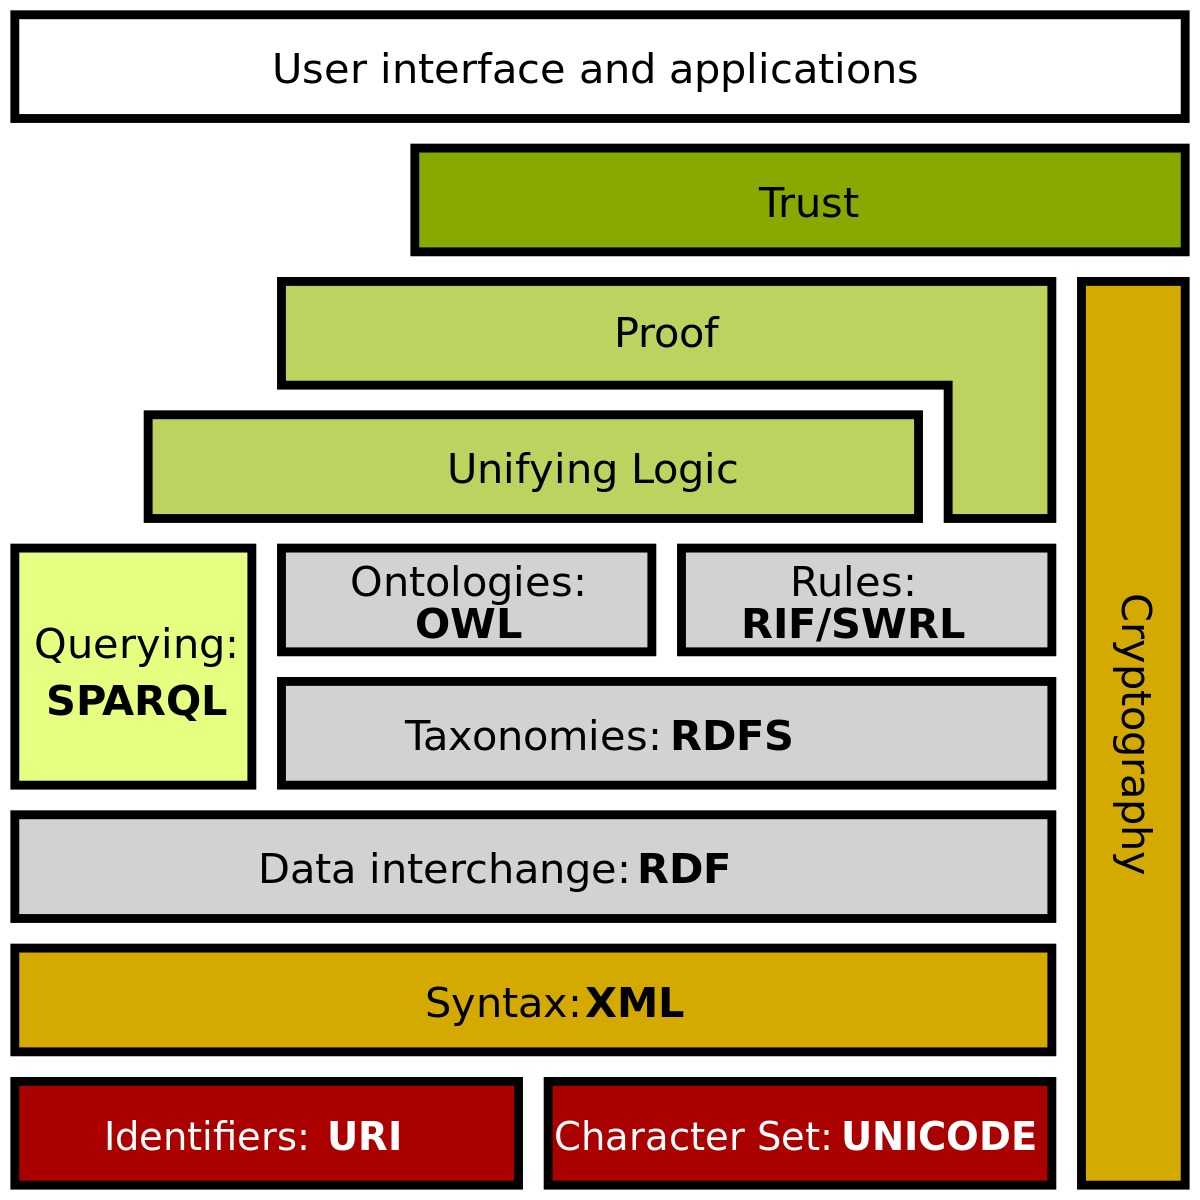
\includegraphics[width=0.45\textwidth]{Figures/Semantic-web-stack.png}
%\end{center}
%\caption{\label{stack} La pile du Web Sémantique}
%\end{figure}

Parmi les technologies utilisées pour exposer des données sur le Web de données RDF, RDFS, OWL et SPARQL sont les éléments importants.\\

\textbf{RDF (Resource Description Framework)} est largement utilisé pour intégrer des données issues de plusieurs sources. Ceci est dû au cadre qu'il fournit pour décrire une ressource et ses relations sous la forme de triplets, Subject-Predicate-Object. Ces triplets peuvent être combinés pour construire un grand réseau d'informations (également connu sous le nom de graphe RDF), intégré à partir de différentes sources de données.  RDF peut être représenté selon differentes syntaxes. L'une des syntaxes (ou sérialisations) de ce langage est RDF/XML. D'autres syntaxes sont apparues ensuite, cherchant à rendre la lecture plus compréhensible. Citons par exemple N3, Turtle, RDFa et plus récemment JSON-LD.\\ 
 
Le langage de requête SPARQL offre aux utilisateurs la flexibilité d'extraire et de manipuler les informations stockées sur plusieurs graphes RDF et même sur plusieurs bases de connaissances distribuées. \\ 

La section \ref{interrogation} donnera de plus amples détails sur la manière de représenter et d’interroger les données liées.
Le rôle du web sémantique dans cette masse de connaissances est de décrire les ressources pour favoriser leur exploitation. Reste qu'une grande partie des descriptions sont écrites en langage naturel qui reste ambigu pour les machines ce qui amène une tentative de solution liée à l'usage d'ontologies (représentant divers concepts biologiques). \\

Dans la section précédente, nous avons survolé les principales composantes du web sémantique : URI, RDF, HTTP et SPARQL. Cette section donnera de plus amples détails sur la représentation et l’interrogation des données structurées et liées.

\subsection{Représentation et interrogation des données}\label{interrogation}

\subsubsection*{Représentation des données}

Les données en web sémantique sont représentées de façon hiérarchique sous forme de triplets RDF dans un multi-graphe orienté étiqueté.\\

Comme illustré à la figure  \ref{triplet}, les graphes sont constitués de sommets et d’arêtes représentant les ressources et les prédicats respectivement. Une fois que la ressource est identifiée par une URI, elle peut être sujette à une question (ou un prédicat) dont la réponse est l’objet qui est lui associé. L’objet peut être sous deux formes : soit une chaîne de caractères soit un URI. Il s’agit d’un litéral ou d’une ressource respectivement.\\

La figure \ref{triplet} représente :
le sujet par l’URI ou la ressource \\ 
\textbf{http://identifiers.org/ensembl.plant/Os01g0100100},
le prédicat indique que ce sujet possède une position chromosomique, — la valeur de l’objet est \textbf{chr01}.

\begin{figure}[!ht]
\begin{center}
	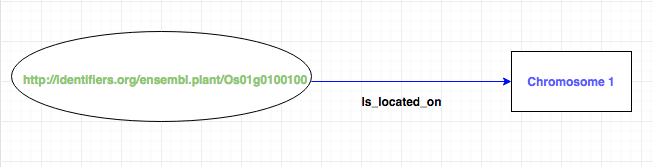
\includegraphics[width=1\textwidth]{Figures/rdf-example.png}
\end{center}
\caption{\label{triplet} Représentation d'un triplet RDF ( {\color{green}sujet}, prédicat, {\color{blue}objet})}
\end{figure}


Le RDF et le \textbf{RDFS (Resource Description Framework Schema)} sont considérés comme les premières fondations de l’interopérabilité sémantique. A la différence du RDF, le RDFS fournit des éléments de base pour la définition d'ontologies ou vocabulaires destinés à structurer des ressources RDF. Il définit notamment la notion de class \textbf{rdfs:Class} et sous-classe \textbf{rdfs:subClassOf} permettant de structurer les ressources RDF de manière hiérarchique. RDFS posède également la propriété \textbf{rdfs:Label} qui permet de nommer une ressource inépendamment de son URI.\\

La figure \ref{RDFS} représente le triplet donné en exemple \ref{triplet} dans le contexte du schéma RDF developpé pour AgroLD (nommé agrold\_vocabulary). La ressource identifiée par \textbf{ensembl:Os01g0100100} est décrite comme appartenant à la classe \textbf{Gene} du vocabulaire AgroLD par la relation \textbf{rdf:type} qui lui même est une sous-classe de la ressource \textbf{obo:SO\_0000704} provenant de l'ontologie Sequence Ontology. Si on utilisait un mécanisme de resonnement sur ces graphes et ontologies, on déduirai par transitivité que \textbf{ensembl:Os01g0100100} aurait aussi comme \textbf{rdf:type} \textbf{obo:SO\_0000704}.\\

Nous avons vu qu’il était possible d’insérer des informations en triplets dans un graphe hiérarchisé pour lier, représenter et publier les données sur le web. Les ressources peuvent être décrites selon un vocabulaire bien déterminé tels que les noms de classes, les types de ressources et les types de relations entre elles. Cependant, le RDFS connait différentes limites dont nous ne citerons que deux exemples:\\
\begin{itemize}
\item la combinaison de classes : il n’est pas possible de montrer que la classe protéine a plusieurs familles,
\item la disjonction : il n’est pas possible de dire que les oxydases et les réductases sont deux sous-classes disjointes.\\
\end{itemize}


\textbf{Le language OWL (Web Ontology Language)} étend le langage RDFS en offrant une meilleure expressivité pour définir des ontologies. Il utilise en effet, une richesse plus importante dans la manière de décrire les concepts et leurs relations à travers son vocabulaire et sa manière de décrire les contraintes en utilisant des propriétés de description de classes telles que des cardinalités, unions, intersections et complémentarités. Lors de la conception d’un ontologie, il est possible d'étendre ou d'intégrer différentes ontologies existantes. Il sera alors nécessaire d'indiquer de quels vocabulaires les termes employés proviennent. Une ontologie est composée de classes, de propriétés et d'instances. Les classes définissent un groupe de sujets ayant des caractéristiques similaires hiérarchisés avec une possibilité d'héritage multiple. Les propriétés expriment des faits sur des individus. Par exemple la position de début et de fin d'un gène et sa localisation chromosomique. Les instances quant à elles, énoncent un axiome d'appartenance à une classe ou concernant l'identité des sujets. Nous ne détaillerons pas plus dans ce mémoire. Grigoris Antoniou et Frank Van Harmelen apportent de plus amples informations sur le langage OWL~\cite{Antoniou2009a}.\\

De grands efforts ont été déployés depuis plus de 10 ans afin de structurer et partager les vocabulaires au sein de la comunauté Biomédicale et des sciences de la vie. Parmi les initiatives les plus importantes citons MGED (Micro Array Gene Expression Data)~\cite{Whetzel2006} qui décrit les données d’expériences de puces à ADN mais surtout OBO (Open Biomedical Ontologies)~\cite{Smith2007,Golbreich2007,Tirmizi2011} qui à travers un format standard (OBO), des outils (OBO Edit) et une plateforme web centralise la majorité des ontologies développées dans le domaine biologique. Le projet a grandement contribué à la démocratisation et l'utilisation massive des vocabulaires controlés et des ontologies dans ce domaine mené en premier lieu par Gene Ontology. Dés lors, de nombreuses plateformes se sont développées afin de fournir un niveau de services important pour utiliser ces ontologies.  Le National Center for Biomedical Ontology’s (NCBO) développe et maintient Bioportal~\cite{Noy2009} une plateforme qui contient plus de 400 ontologies et terminologies biomédicales. Ontobee~\cite{Ong2016} permet de faciliter le partage d’ontologies, l’intégration et l’analyse des données ainsi que leur visualisation et leur requêtes. Le Ontology Lookup Service (OLS)~\cite{Cote2006} fournit un accés aux ressources OBO utilisé par la plateforme génomique de l'EBI (European Bioinformatics Institute).\\

Comme je l'ai déjà mentionné, les nouvelles technologies de production de données haut-débits en médecine et en biologie génèrent de grands volumes de données. En plus de ce phénomène qui touche également d'autres secteurs professionnels, s'ajoute l’hétérogénéité et la diversité et complexité des données qui sont les principaux problèmes abordés en bioinformatique. La recherche, le tri et l’accès aux données, leur interprétation et leurs annotations sont des tâches fastidieuses à réaliser pour un expert biologiste.  Les technologies du web sémantique offrent des solutions prometteuses pour ces domaines puisqu'il vise à faire participer à la fois les utilisateurs et les machines~\cite{berners2001semweb}.\\

Dans le web sémantique, il existe différentes bases de connaissances qui sont regroupées en fonction du domaine d'expertise. MeSH (Medical Subject Headings)\footnote{\url{https://www.nlm.nih.gov/mesh}} est une terminologie biomédicale trés utilisée dans le domaine scientifique et également transformée pour le web de données. MeSH est le trésor de termes de référence permettant d’indexer, rechercher et classer des documents tels que ceux de PubMed et bien d'autres bases de données dans le domaine biomédical. Aujourd'hui, c'est la ressource la plus utilisée et reliée aux autres ressources. En 2009, il a été recensé pour le domaine des sciences de la vie 191 millions de "liens sortant" 4 et plus de 3 milliards de triplets RDF soit environ 10\% du total. Aujourd'hui, il en représente 30\% pour tous les domaines confondus. De plus, l’ensemble de jeux de données liées a été multiplié par 8 en l'espace de 10 ans : il passe de 41 à 332 sur un total de 1163. Ces données liées structurées sont consultables directement en ligne et téléchargeables\footnote{\url{http://lod-cloud.net}}. Elles sont pour la majorité mises à jour régulièrement. Max Schmachtenberg et ses collaborateurs ont recensé en avril 2014 l'état des ressources disponibles et plus récemment Andrejs Abele et al. Une vue d’ensemble est présentée en fonction des domaines, du nombre d’ensembles de données, de triplets et des liens les reliant~\cite{Schmachtenberg-al2014}.\\

\begin{figure}[!vt]
\begin{center}
	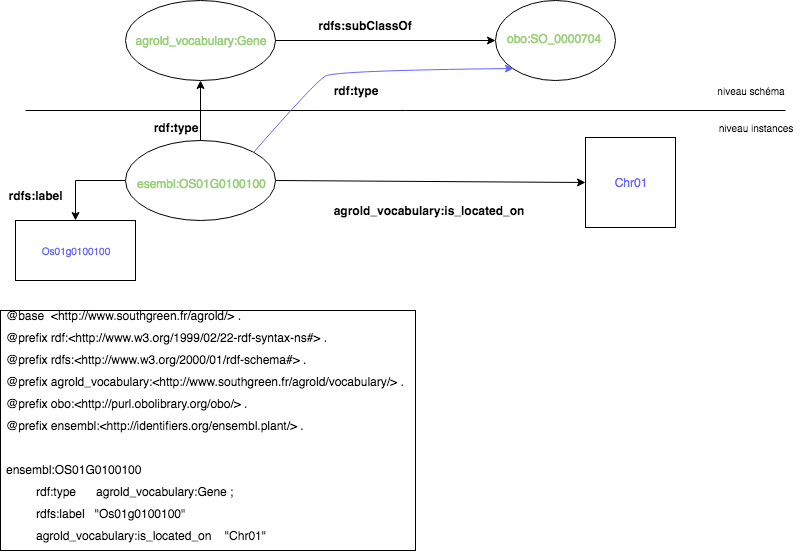
\includegraphics[width=1\textwidth]{Figures/RDF-into.png}
\end{center}
\caption{\label{RDFS} Représentation d'un schéma RDFS }
\end{figure}



\subsection{Extraction de connaissances biologiques}

Le constat établi est que les ressources issues de bases de données restent limitées pour produire une connaissance suffisante et nécessaire pour formuler des hypothèses de recherche d’information sur les fonctions moléculaires des gènes et leurs rôles dans l’expression de phénotype. Il existe des ressources annotées manuellement comme OryzaBase ou Qtaro (pour ne citer qu'un petit nombre) mais elles ne fournissent pas un contenu exhaustif de l'information et ont un délais de mises à jour plus long. \\

Dans le domaine de l’extraction de connaissances, une tâche importante consiste à identifier et classer par type les entités biologiques, également appelée des entités nommées\footnote{named entity recognition (NER)} .

\subsubsection{Méthodes d'extraction d'entité nommées}
La tache la plus importante dans le domaine bioinformatique concerne l'extraction d'entitées nommées (Named Entities Recognition  - NER) telles que les nom de gènes, protéines, d'espèces, mutants ou de composés biochimiques. De plus l'extraction de structures plus complexes telles que les relations  et les évènements entre entités dépend de la capacité à détecter ces dernières. De fait, le domaine bénéficie d'une longue expérience en la matière, dont les conférences  \textbf{Biocreative} \footnote{Biocreative - \url{http://www.biocreative.org}}, \textbf{BioNLP}\footnote{\url{http://2016.bionlp-st.org}} en sont les vitrines depuis 2004.\\
Plusieurs méthodes et outils de fouille de texte ont été développés dans la littérature pour résoudre ce problème. Elles sont répartis en quatre approches principales~\cite{Basaldella2017} : i)  utilisant un dictionnaire de mots, ii)  à base de règles écrites manuellement, iii) utilisant des approches de machine learning, iv) approches combinant le machine learning et au moins une des deux autres.\\

Les méthodes basées sur un dictionnaire, l'une des approches bioinformatique les plus fondamentales du NER, utilisent des listes complètes de termes afin d'identifier les occurrences d'entités dans le texte. Toutefois, compte tenu de l'évolution rapide et constante des découvertes scientifiques, il est difficile de maintenir à jour des listes de dictionnaires. De plus, l'abondance de synonymes (i.e. la même entité peut avoir deux noms differents) ou l'utilisation fréquente d'acronymes - MONOCULM (MOC) - complexifie la tâche d'identification et d'association à des entités existantes. Ces méthodes sont donc aujourd'hui associée à d'autres approches~\cite{Hettne2009,Gerner2010}. \\

Une autre approche consiste à définir des règles basées sur des modèles qui exploitent les caractéristiques orthographiques et lexicales des classes d'entités ciblées afin de les reconnaître (par exemple pour les protéines~\cite{Franzen2002}). Parce qu'il nécessite une expertise humaine et nécessite beaucoup de travail pour créer de tels modèles, les systèmes ultérieurs essaient d'apprendre automatiquement de tels modèles à partir de données étiquetées~\cite{Califf1999,Ciravegna1999}. Des travaux plus récents sur la reconnaissance d'entités nommées utilisent des méthodes statistiques d'apprentissage automatique qui peuvent etre combiner aux méthodes précédentes. \\

Au cours des dernières années, les 2 méthodes précédentes ont été remplacées par des approches basées sur l'apprentissage automatique supervisé, en particulier les algorithmes de classification séquentielle, tels que les modèles de Markov cachés~\cite{Rabiner1989} et les CRF~\cite{Lafferty2001}. Les CRF sont devenus le modèle standard de facto~\cite{Settles2004}, étant la méthode de choix pour la quasi-totalité des outils ayant remporté des compétitions récentes de type NER, comme BioCreative IV~\cite{Krallinger2013} ou i2b2~\cite{Uzuner2011} . Les outils NER populaires utilisant les CRF sont, par exemple, ABNER (A Biomedical Named Entity Recognizer)~\cite{Settles2005} et BANNER~\cite{LEAMAN2007}.\\
Les méthodes hybrides combinent des méthodes d'apprentissage automatique avec des techniques basées sur des dictionnaires ou des règles. Par exemple, ChemSpot~\cite{Rocktaschel2012} intègre les résultats d'un modèle CRF avec un module d'appariement de dictionnaire pour NER chimique.\\

Récemment, l'utilisation d'approches de réseaux de neurones combinés aux CRF dans l'analyse de texte montre des résultats bien meilleurs qu'avec les approches précédentes ~\cite{Segura-Bedmar2015}. Notamment, les modèles LSTM-CRF (Long Short Term Memory model combinés avec Conditional Random Fields )~\cite{Lample2016} offrent des résultats encourageants. Cependant, ces méthodes nécessitent un volume de données important afin d'optimiser les phases d'entraînements~\cite{Habibi2017a}. \\


Afin d’en extraire de l’information pertinente, ici les entités Ehd1, Hd3a, Ghd7 et Hd1 et la relation down-regulated, je souhaite evaluer des approches de « text mining » (NLP). notamment les récents développement qui utilisent les méthodes de deep learning avec des modèles LSTM-CRF (Long Short Term Memory model combinés avec Conditional Random Fields ) pour détecter les Entités Nommées~\cite{Habibi2017a,Basaldella2017}. L’accent sera également donné sur la constitution d’un corpus de données sur le riz qui pourra servir de modèle d’entrainement pour détecter des Entités et leurs relations dans le texte. Le but de ce travail sera de proposer un module d'extraction d’information et formalisation de connaissances que les experts puissent valider par l’application AgroLD. 
% parler de l ontologies AgroLD de la detection de relations


\section{Objectifs}
\label{Objectifs}

%verifie la ponctuation
Mon projet de recherche aborde le problème suivant : Comment gérer et structurer la complexité des données biologiques afin d’en extraire de la connaissance permettant d’identifier les mécanismes moléculaires contrôlant l’expression de phénotypes chez les plantes. 
L’objectif de ce projet sera de déterminer si la représentation d’information sous forme de graphes de connaissances est adaptée pour formuler des hypothèses de recherche permettant de lier le génotype au phénotype En prenant le riz comme modèle, l’objectif de ce projet est de construire des réseaux d’interaction moléculaires entre gènes à partir de données éparses (articles scientifiques, bases de données publiques, données expérimentales, …) afin d’identifier les gènes clés pour l’amélioration des plantes. Compte tenu de l’ambition du projet, je compte organiser mon travail dans des activités qui seront menés en parallèles sur une durée de 5 ans. Chacune de ces activités propose de traiter (voire résoudre) des verrous scientifiques relevant des domaines informatique et bioinformatique. Par ailleurs, je compte obtenir des financements sur appels d’offres pour développer ces activités sur un plus long terme. \\

Dans un premier temps afin d'aborder la question initiale, comment intégrer ces données diverses pour faciliter l’identification de gènes importants pour les biologistes,  plusieurs pistes de recherche regroupées en trois grandes voies : Intégration dynamique des données, enrichissement des connaissances, priorisation de gènes candidats. Dans ce processus, 1) une première voie consistera à transformer et intégrer dynamiquement ces données dans AgroLD pour les rendre plus facilement utilisables en termes algorithmique. Une attention particulière sera portée aux données expérimentales produites par les chercheurs des unités plantes Montpelliéraines (DIADE, AGAP, IPME) et les partenaires du sud (LMI RICE, IRRI). S’agissant souvent de données massives (i.e. données de génotypages ou d’images), la méthode proposée évitera de transformer intégralement les données afin de garantir de bonnes performances, 2) une deuxième voie consistera à proposer de nouvelles méthodes d’annotation sémantique pour lier plus facilement différentes sources de données avec les concepts ontologiques et en extraire des informations. Nous utiliserons de nouvelles fonctionnalités d’Agroportal un portail d'ontologies de référence pour le domaine agronomique,  3) une troisième voie consistera à développer des méthodes de fouille de texte pour identifier les entités biologiques et leurs relations dans les publications scientifiques.\\


\begin{figure}[!ht]
\begin{center}
	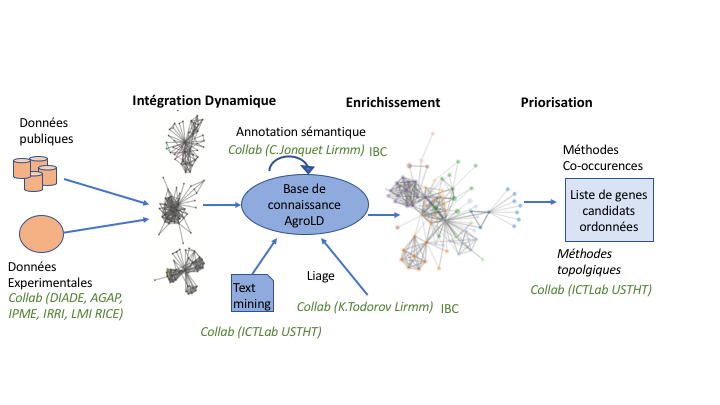
\includegraphics[width=0.9\textwidth]{Figures/schema-projet-recherche.png}
\end{center}
\caption{\label{schema-general} Schema général du projet de recherche}
\end{figure}

Ces différentes approches permettent d’extraire des informations et de lier les données sous forme de graphes de connaissances (on parle de graphe RDF). 4) Pour enrichir les liens entre les différents graphes générés et ainsi produire un réseau d’interaction qui permettra la découverte de nouvelles connaissances, une méthode de liage de données RDF spécifique aux problématiques bioinformatique sera développée. Enfin, afin de permettre une recherche d’information efficace et trier pertinemment les résultats, 5) plusieurs méthodes et algorithmes de priorisation de gènes candidats seront évaluées et proposées. \\




\section{Intégration de données et extraction de connaissances}




\subsection{Intégration dynamique des données}

La première étape du développement du graphe de connaissance sera d’intégrer et de transformer en RDF de nouvelles ressources pour le riz afin de construire un large réseau d’interaction moléculaire (réseaux de co-expression de gènes, transcriptomique, Facteur de transcriptions, complexe proteine-proteine). Ce processus de transformation est souvent appelé le \textbf{lifting de données}. Je m’appuierai sur le projet AgroLD (Agronomic Linked Data) une base de connaissance que je développe activement depuis 2015 dans le cadre du projet investissement d’avenir Institut de Biologie Computationnelle (IBC). Dans ce contexte, j'ai eu l'occasion de developper de nombreux outils de lifting soit pour des sources spécifiques (e.g.  TropGeneDB, OryzaTagLine, etc.) soit pour des formats de fichier génériques (e.g. GAF, VCF, GFF, etc.). \\

Toutefois, une attention particulière sera portée aux données expérimentales produites par les chercheurs de l’unité Diade ou les partenaires du sud (LMI RICE, IRRI). S’agissant souvent de données volumineuses (i.e. données de génotypages ou d’images), la méthode doit éviter de transformer intégralement les données afin de garantir de bonnes performances.\\

Concernant l'extraction d'information contenue dans des bases de données relationnelles, nous avons développé une application BioSemantic, au cours de la thése de Julien Wollbrett. Cette derniere propose une approche flexible et automatisée pour la creation de vue RDF en se basant sur D2RQ  et assiste l'utilisateur dans la formulation de requêtes se basant sur ces vues en développant un algorithme de recherche de plus court chemin dans les graphes RDF~\cite{wollbrett2013clever}. Toutefois, il existe de nombreux outils de transformation et language de mapping associés adaptés aux différents types de SGBD et aux modèles de représentation des données. L'article de Michel et al~\cite{Antipolis2014} en dresse un inventaire et compare les différentes méthodes. De plus, les auteurs proposent également  le langage xR2RML~\cite{Michel2015} qui présente l’avantage de transformer les données à la demande au cours d’une requête et ce pour un differents types de bases de données (XML, object-oriented, NoSQL). En collaboration avec l’équipe Inria wimmics, je compte développer ces aspects pour extraire les données expérimentales de variations génomiques actuellement stockées dans Gigwa~\cite{Sempere2016}. Gigwa est une application que nous développons avec Guilhem Sempéré et qui permet de gérer de grands volumes de données pour l’analyse de variations génomiques.


\subsection{Annotation sémantique}

Ainsi, dans cette première phase de transformation, chaque graphe RDF produit est indépendant des autres. C’est grâce aux ontologies que les liens sémantiques entre les entités biologiques peuvent être créer. Dans notre domaine, le cadre conceptuel pour la gestion des connaissances est basé sur des ontologies bien établies : Gene Ontology, Sequence Ontology, Plant Ontology(PO), Trait Ontolgy (TO), Phenotype quality ontollogy (PATO) et Environnement Ontology (OE). Un lien sémantique (e.g. annotation sémantique) est créé des lors qu’une entité biologique référence un terme ontologique (e.g. la protéine IAA16 est exprimée dans « le coléoptile » qui a pour URI OBO:PO\_0020033). Ainsi, il est possible de relier des entités d’un même graphe ou dans des graphes différents dès lors qu’elles partagent les mêmes liens sémantiques. Dans AgroLD, nous exploitons les annotation sémantiques lorsqu’elles sont explicitement présentes dans les jeux de données (e.g. un gène est annoté dans une ressource avec le terme GO :xxxxx). Cette méthode nous permet de produire 22 \% d’annotations supplémentaires. Toutefois, de nouvelles méthodes doivent être développées pour les nombreuses ressources qui ne possèdent pas ces informations.\\

Identifier des liens sémantiques dans les données est un élément important pour la construction des réseaux de connaissance dans AgroLD. C’est également un champ disciplinaire très actif dans la communauté informatique~\cite{Faria2013,Otero-Cerdeira2015} . De fait, de nombreuses méthodes sont proposées afin de relier des termes (ou concepts) issus de différentes ontologies mais peu proposent des méthodes efficaces dans le cas de traits complexes comme les maladies ou les phénotypes~\cite{harrow2017}. Dans notre cas, il y a certaines spécificités dont il faut tenir compte : \\


\begin{itemize}
\item Un terme (le  peut faire référence à plusieurs ontologies de domaine differents (e.g. Dwarfism -> PATO, Tillering -> PO, Tiller angle -> TO),
\item Un terme composé peut être annoté à partir de deux ontologies (e.g. wrinkled seed, aborted seed font référence aux ontologies PATO et PO),
\item Un terme biologique peut être representé par son symbole ou son acronyme,
\item Un terme biologique peut être polysémique et ambigu, donc difficile à annoter,\\
\end{itemize}

Pour répondre à ces défis et d'autres liés à l'analyse de textes biologiques non structurés, les outils d'annotion sémantiques performants reposent souvent sur une utilisation combinée de traitement de texte, de bases de connaissances, de mesures de similarité sémantique et de techniques d'apprentissage automatique~\cite{Jovanovic2017a}. Agroportal~\cite{Jonquet2018} vise à développer un portail d'ontologies de référence pour le domaine agronomique. Le portail ambitionne également de proposer plusieurs outils de recherche et d'annotation sémantique. Comme indiqué dans (Jonquet et al, 2018)~\cite{Jonquet2018}, nous comptons développer un workflow d’annotation entre AgroPortal et AgroLD basé sur des mesures de similarités, le traitement de texte (voir section \ref{NLP}) et utilisant les fonctionnalités d’AgroPortal pour réaliser l’association des données avec les concepts ontologiques. \\

Il arrive également que dans certains cas les différentes ontologies utilisées ne se recouvrent pas. Afin de relier les différents types de données et propriétés de ces ontologies, j'ai initié le développement d’une ontologie AgroLD qui servira de glu entre les classes et les propriétés identifiées dans AgroLD\footnote{\url{https://github.com/SouthGreenPlatform/AgroLD_ETL/blob/master/model/agrold\_schema.rdf}}. \\


\section{Enrichissement de la connaissance et fouilles de données dans les graphes}

\subsection{Extraction d’entités biologiques et de relations}
\label{NLP}

Le constat établi est que les ressources issues de bases de données restent limitées pour produire une connaissance suffisante et nécessaire pour formuler des hypothèses de recherche d’information sur les fonctions moléculaires des gènes et leurs rôles dans l’expression de phénotype. Il existe des ressources annotées manuellement comme OryzaBase ou Qtaro (pour ne citer qu'un petit nombre) mais elles ne fournissent pas un contenu exhaustif de l'information et ont un délais de mises à jour plus long. Un des enjeux du projet sera d'enrichir AgroLD à partir des données non-structurées qui sont contenues dans les publications scientifiques et dans des champs textes des bases de données (par exemple les champs « commentaires », « descriptions »). Nombre de ces champs contiennent, des mécanismes moléculaires et génétiques d’intérêts qui sont souvent décrits par des expressions complexes associant des entités biologiques reliées par des relations sémantiques spécialisées (e.g. \textit{Ehd1 and Hd3a can also be down-regulated by the photoperiodic flowering genes Ghd7 and Hd1}).\\

\textbf{Dans le domaine de l’extraction de connaissances}, une tâche importante consiste à identifier et classer par type les entités biologiques, également appelée des entités nommées\footnote{named entity recognition (NER)} . Plusieurs méthodes et outils de fouille de texte ont été développés dans la littérature pour résoudre ce problème. Elles sont répartis en quatre approches principales~\cite{Basaldella2017} : i) à base de règles écrites manuellement, ii) utilisant un dictionnaire de mots, iii) utilisant des approches de machine learning, iv) approches combinant le machine learning et au moins une des deux autres. Nous avons évalué l’état de l’art des approches de NER, dans l'objectif d’enrichir des données liées avec de l'information extraite à partir des champs littéraux des graphes RDF ou des articles scientifiques.  approches 

L'architecture de LSTM-CRF est illustrée à la figure\ref{LSTMCRF} \cite{Habibi2017a}. L'ensemble du système comprend trois couches principales: la couche d'intégration en entrée, la couche bidirectionnelle LSTM et la couche CRF en sortie. A partir d'une phrase composée de la séquence de mots $ w_ {1} $; $ w_ {2} $; ...; $ w_ {n} $ en entrée, la couche d'intégration produit un vecteur d'intégration $ x_ {1} $; $ x_ {2} $; ...; $ x_ {n} $ pour chaque mot. Chaque vecteur d'inclusion concernant un mot distinct est une concaténation de deux composants: l'inclusion au niveau du mot et du caractère. Nous cherchons les vecteurs d'inclusion de mots à partir d’une table de recherche de vecteurs d'inclusion de mots. En même temps, nous appliquons un LSTM bidirectionnel à la séquence d'inclusion de caractères pour chaque mot, puis concaténons les deux sens pour obtenir l'inclusion au niveau du caractère. Cela signifie que la séquence d'inclusion résultante  $ x_ {1} $; $ x_ {2} $; ...; $ x_ {n} $ est introduite dans la couche LSTM bidirectionnelle afin de produire une représentation plus précise de la séquence d'entrée et passe ensuite en entrée de la dernière couche CRF. La sortie finale de cette couche est obtenue en appliquant l'algorithme classique de Viterbi. 

\begin{figure}[!ht]
\begin{center}
	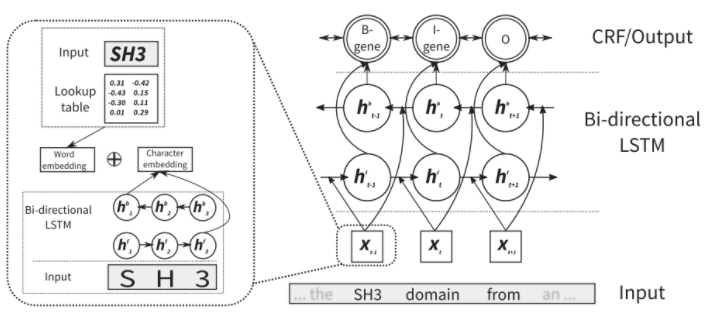
\includegraphics[width=1\textwidth]{Figures/LSTMCRF.png}
\end{center}
\caption{\label{LSTMCRF} Le modèle LSTM-CRF présenté dans \cite{Habibi2017a}}
\end{figure}

L'approche hybride~\cite{Basaldella2017} repose sur un dictionnaire d'entités associé à des classificateurs d'apprentissage automatique. Dans un premier temps le dictionnaire de recherche d’entités OGER (OntoGene Entity Recognizer) est utilisé pour annoter les objets dans les ontologies de domaine sélectionnées. Il s'agit d'un service web qui fournit un accés aux dictionnaires construits sur les bases pubmed du NCBI\footnote{https://www.ncbi.nlm.nih.gov/pubmed}. Ensuite, le framework Distiller est utilisé pour extraire ces informations en tant que fonctionnalité permettant à un algorithme d’apprentissage automatique de sélectionner des entités pertinentes. Le processus de Distiller est basé sur une extraction automatique de mots clés (AKE) pour extraire des informations d’un texte. AKE semble être différent de NER, car celui-ci s'intéresse a la recherche du petit ensemble d'information les plus pertinentes dans un document, puis par la recherche de toutes les informations des types sélectionnés. En outre, AKE peut être exécuté à la fois en tant qu’algorithme non supervisé et supervisé, et Distiller tire réellement son origine d’une approche non supervisée. 
En ce qui concerne son architecture, Distiller est organisé en une série de modules, chaque module étant conçu pour effectuer efficacement une tâche unique~\cite{basaldella2015introducing}, telle que le part-of-speech (POS), l'analyse statistique, etc. Il fonctionne avec la possibilité d'implémenter différents pipelines pour différentes tâches. Les modules partages leur informations sur les entités dans une mémoire partagée afin que les autres modules puissent y accéder. L'implémentation d'une tâche d'extraction avec Distiller conduit à la spécification d'un pipeline associant les modules. Une tâche d'extraction est normalement divisée en étapes: pré-traitement, sélection de phrase clé candidate et classement de candidats. Le schéma du pipeline Distiller est décrit à la figure \ref{distiller}.

\begin{figure}[!ht]
\begin{center}
	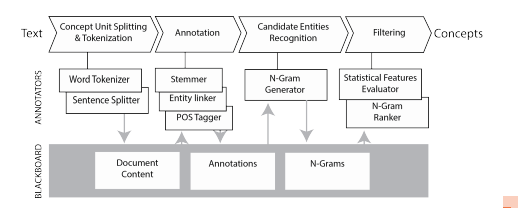
\includegraphics[width=1\textwidth]{Figures/distiller.png}
\end{center}
\caption{\label{distiller} Le schéma du Distiller présenté dans ~\cite{Basaldella2017}}
\end{figure}

Pour l'évaluation de cette approche, nous avons mis en œuvre deux algorithmes d’apprentissage automatique différents: les réseaux de neurones (NN) et les CRF. Les performances du Distiller sont différentes en fonction du modèle utilisé. Dans le cas de CRF, il utilise la sortie annotée d'OGER en tant que propriété et considère tout élément dans le texte comme une entité à prédire. En revanche, Distiller utilisé seul se concentre uniquement sur le filtrage de la sortie d'OGER et sur le processus de classification pour chaque entité. Pour résumé, nous avons implémenté 3 méthodes pour évaluer l'approche hybride: \\
\begin{itemize}
\item basée sur les résultats OGER
\item basée sur un post-traitement des résultats d'OGER avec des réseaux de neurones (NN) 
\item basée sur un post-traitement des résultats d'OGER avec CRF\\
\end{itemize}


Dans ce projet, nous avons utilisé les jeux de données de Oryzabase \footnote {\url{https://shigen.nig.ac.jp/rice/oryzabase/}}, une base de données intégrée sur le riz. En nous focalisant sur les gènes du riz, nous avons téléchargé les jeux de données Gene List et Reference contenant respectivement une liste de 21739 gènes différents connus et un ensemble de résumé d'articles avec des gènes associés. Nous les avons utilisé comme données d'entrainement et de validation, respectivement pour les diverses approches d'extraction d'entités.

Nous avons évalué les performances de tous les modèles sur le jeu de données Oryzabase. Les résultats en termes de précision, rappel, $ F_ {1} -score $ pour chaque modèle sont présentés dans le tableau \ref{result1}. LSTM-CRF réalise les meilleures performances parmi les modèles. En moyenne, le score $ F_ {1} $ - est égal à 86,72 \% pour la méthode générique LSTM-CRF et à 80,44 \% pour la méthode générique LSTM.

\begin{center}
\begin{table}[h]
\begin{tabular}{ |p{2.5 cm}| p{1.5 cm}|p{1.5 cm}|p{1.5 cm}|p{1.5 cm}| p{1.5 cm}|p{1.5 cm}|} 
\hline
\multirow{2}{4em}{} & 
\multicolumn{2}{|c|}{Precision(\%)} 
& \multicolumn{2}{|c|}{Recall(\%)}
&\multicolumn{2}{|c|}{$F_{1}-score$(\%)} \\&
(i)&(ii)&(i)&(ii)&(i)&(ii) \\
\hline
LSTM & 80.16& 78.06& 79.16&82.97&79.66 &80.44 \\ 
\hline
LSTM-CRF &87.24&87.32&84.73&86.13&85.97&86.72 \\
\hline
\end{tabular}
\newline
\caption{\label{result1} le résultat des performances en termes de précision, de rappel et de $ F_ {1} -score $ pour les méthodes LSTM et LSTM-CRF avec différents paramètres d’entraînement: (i) learning rate = 0,001, dropout = 0,3, (ii) learning rate = 0,001, droupout = 0,5}
\end{table}
\end{center}

D'un autre côté, le résultat de la méthode hybride est très exploitable. La performance de OGER avec CRF a donné le meilleur résultat parmi les 3 tests, soit 86,72\% en moyenne. Le deuxième correspond à OGER associé au réseau de neurones, qui a atteint une précision de 67\% en moyenne. Bien que les améliorations ne soient pas aussi élevées que prévu, il y a eu quelques améliorations, comparé à OGER seul qui se situe autour de 58,5 \%. Le résultat est présenté dans le tableau \ref{resultat2}.

\begin{center}
\begin{table}[h]
\begin{tabular}{ |p{2.5cm}|p{3 cm}| p{3 cm}|p{3 cm}|} 
\hline
 &Precision(\%)&Recall(\%)&$F_{1}-score$(\%)\\
 \hline
OGER&53.03&65.23&58.50\\ 
\hline
OG+NN& 63.93&71.10 &67.32 \\
\hline
OG+CRF & 88.39&82.24&85.08\\
\hline
\end{tabular}
\newline
\caption{\label{resultat2} le résultat des performances de la méthode hybride en termes de précision, de rappel et de $F_{1}-score$}
\end{table}
\end{center}

\subsection{Liage des données}

Un second élément important dans l’enrichissement est le liage (l’interconnexion) de données. Le processus qui peut avoir plusieurs designations anglophones, \textit{instance matching}, \textit{data linking} et \textit{link discovery} vise à établir des liens sémantiques d’équivalence entre les entités de graphes différents. Il vise à déterminer si deux ressources données se réfèrent ou non au même objet du monde réel. La problématique de liage est un domaine de recherche actif qui a introduit une pléthore d'approches. De fait, de nombreux outils ont été développés pour traiter ce problème au cours des dernières années. Ces approches et outils ont été étudiés dans~\cite{ferrara2011,Achichi2016,erv271}. 
La majorité des infrastructures de liage actuelles utilisent généralement des workflows composés de plusieurs étapes afin d'effectuer le liage. Dans la plupart des cas, ces workflows sont des instanciations du workflow générique présenté à la figure \ref{liage1}. Les paramêtres en entrée incluent en général les deux jeux de données à lier (source, cible), les paramètres de configuration et les ressources externes qui peuvent être facultatives. Les données d'entrée peuvent être fournies sous la forme de dump RDF / OWL ou sous la forme d'un SPARQL endpoint pour un accès aux données basé sur une requête. Le liage peut être restreint à un sous-ensemble d'une source de données, par exemple des instances d'une classe particulière et il n'est pas nécessaire de les comparer à des entrepôts de données plus génériques tels que DBpedia. Les paramêtres de configuration peuvent être des règles de liage ou des mesures de similarité pour établir des liens d'identité. Les données d'entrainements peuvent etre fournies pour des étapes de liage basés sur l'apprentissage. D'autres outils peuvent éventuellement être utilisés comme d'autres sources de connaissance, par exemple, des dictionnaires de données ou des mappings préalablement définis. La sortie du workflow est un ensemble des liens trouvés ou des correspondances représentant un liage entre les jeux de données source et cible en général déclaré avec des predicats \textit{owl:sameAs}.


\begin{figure}[!ht]
\begin{center}
	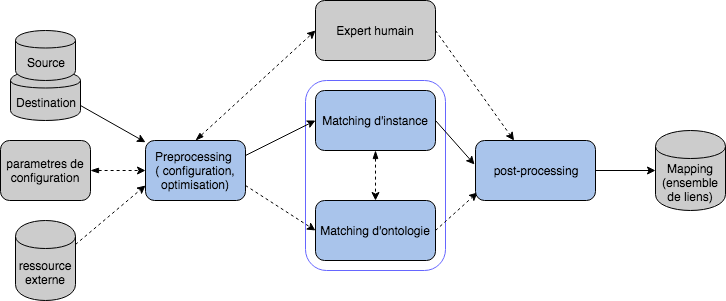
\includegraphics[width=1\textwidth]{Figures/liage.png}
\end{center}
\caption{\label{liage1} Workflow général du processus de liage de données adapté de~\cite{erv271} }
\end{figure}

\paragraph{Les challenges du liage de données}
Il existe de nombreux outils qui tendent a résoudre ce probleme mais dans la réalité, le liage de données est un processus complexe et souvent dependant d'un domaine de connaissance. Dans ce processus, l'un des défis consiste à gérer les jeux de données avec un chevauchement limité en termes de propriétés utilisées pour décrire leurs ressources, ce que nous appelons des \textit{jeux de données complémentaires}. Cette information manquante fait qu'il est difficile pour les systèmes récents basés uniquement sur l'analyse des propriétés~\cite{Jentzsch,Ngomo2011} d'évaluer les relations entre instances. Les jeux de données intégrés dans AgroLD presentent largement ce problème. \\

L’exemple \ref{exempleL} montre 2 entités issues de 2 jeux de données différents. Ces entités correspondent à la protéine APO1 mais elles sont considérés comme différentes car elles n’ont pas le même URI. De plus la tache est d'autant plus difficile lorsque les propriétes qui les décrives sont hétérogenes. Une des questions est d'identifier les propriétes sur les se baser pour faire la comparaison. Mais également de déterminer comment les attributs sont valués ou structurés afin d'eviter de produire des liaisons erronées ou de manquer des liaisons. Comme le montre la figure  \ref{liage} , les descriptions peuvent être exprimées dans différents langues naturels, avec différents vocabulaires ou avec différentes valeurs. Ces limitations dans la comparaison peuvent classées selon 3 dimensions: basée sur la valeur, ontologique et logique. \\


\textbf{\textit{La dimention basée sur la valeur}} fait référence aux propriétés contenant des valeurs litérale (texte) exprimée en language naturel ou valeurs numériques et qui peut induire des erreurs de liage. Les auteurs de  ~\cite{achichi2018} identifient 4 niveaux d'hétérogénéité également indiqué dans la figure: terminologique, linguistique, bonnes pratiques de représentation et sur les types de valeurs.\\

\begin{itemize}
\item \textit{Hétérogénéité terminologique.} Dans ce cas les variations vont concerner un terme correspondant a un mot ou un groupe de mots. Cette variation peut s'exprimer de différentes manieres; i) la synonymie lorsque des termes differents vont representer le meme concept; ii) la polysemie lorsque les termes similaires ont des sens differents; iii) des acronymes et abbreviations. Comme on peut le constater sur la figure \ref{liage} un des noms des entités correspond a une abbreviation. Pour palier ce probleme, certaines application proposent des fonctionnalités d'expansion d'acronymes/abbreviations.\\
\item \textit{Hétérogénéité linguistique.}  Les termes concernés sont représentés dans des languages différents. C'est un problème trouvé fréquemment lorsqu'on travaille avec des données experimentales et qui reflètent la diversité des informations que l'on peut trouver sur le web. Dans ce cas, s'agissant de l'anglais et du Japonais, les outils de recherche par simlarité sont inefficace. Il faut passer par une étape de traduction automatique au préalable. \\
\item \textit{Bonnes pratiques de représentation.} La représentation des connaissances est soumise à des bonnes pratiques de conception. Leur transgression est un frein dans la découverte de correspondances.\\
\item \textit{Types de valeurs.} Cette hétérongénéité concerne la manière dont les valeurs sont encodées (e.g. string, integer, etc.). Dans ce cas, le challenge réside dans l'uniformisation des types de valeurs, par exemple uniformiser les dates, les mesures numeriques, etc.\\
\end{itemize}

\textbf{\textit{La dimension ontologique}} fait référence aux variations de classes ou de propriétés associées aux instances comparées. Quatre niveaux d'hétérogénéité sont identifiées: vocabulaire, structure, pronfeur de nivau des propriétés et des descriptions.\\
\begin{itemize}
\item \textit{Hétérogénéité du vocabulaire.} Les classes et les propriétés sont souvent décrites en utilisant différents vocabulaires par différents producteurs de données, car la sémantique d'une classe ou d'une propriété donnée peut être interprétée différemment selon son application. Ce problème est encore plus compliqué dans le contexte du Web de données où toutes les ressources ne sont pas nécessairement décrites de la même manière. L'utilisation de mapping entre vocabulaires, par exemple avec LOV ou Agroportal dans notre cas, peut permettre de dépasser ce problème.\\
\item \textit{Hétérogénéité de la structure.} La description d'une entité peut se faire à différents niveau de granularité. Dans notre exemple le terme Fbox 5-25 est decrit differemment dans les deux entités. Dans ce cas, l'information est incluse dans une structure de données pour la première entité et dans un litéral pour la deuxième. L'utilisation de méthodes NLP pour extraire de l'information sur la deuxième entité peut aider pour le liage.\\
\item \textit{Hétérogénéité de la profondeur de niveau des propriétés.} Elle se situe au niveau du schéma des ressources et correspond à des différences de modélisation des propriétés. Dans notre cas, le litteral \textit{DNA Binding}, qui est une fonction moléculaire, est modélisé à partir d'une classe de type GO pour la premiere entité et une propriété pour la deuxième. La distance entre les deux éléments est donc plus importante pour la première. Les méthodes pour résoudre ce type de problème, peuvent etre d'indexer les litéraux avec leur contexte afin de pouvoir les comparer.\\
\item \textit{Hétérogénéité descriptive.} Une ressource peut avoir plusieurs concepts ou peut être décrite avec un ensemble de propriétés plus important, dans un jeux de données que dans un autre, comme nous pouvons le voir dans notre exemple (voir la figure \ref{liage}). On peut remarquer que ces ressources, et c'est le cas de manière générale, contiennent plus d'information descriptives (des champs litteraux de type texte) que par l'ensemble de propriétés qui les décrivent. Il est évident que comparer ces ressources uniquement par leur propriétés sera moins efficace que des approches prenant en compte l'ensemble des informations. \\

\end{itemize}

\textbf{\textit{La dimension logique}} fait référence au fait que l'équivalence entre deux informations sur deux jeux de données est implicite, mais peut être déduite à l'aide de méthodes de raisonnement. Deux principaux problèmes d’hétérogénéité sont identifiés:\\
\begin{itemize}
\item \textit{Hétérogénéité de classe.} Ce type d'hétérogénéité concerne le niveau de la hiérarchie des classes. C'est généralement le cas de deux ressources appartenant à des classes différentes pour lesquelles une relation hiérarchique explicite ou implicite est définie (les concepts «Protein» et «Enzyme», dans la figure  \ref{liage}, illustrent ce problème). De plus, deux instances se rapportant au même objet peuvent appartenir à deux sous-classes différentes de la même classe.\\
\item \textit{Hétérogénéité de propriété.} A ce niveau, l'équivalence entre deux valeurs est déduite après l'exécution d'une tâche de raisonnement sur les propriétés. Deux ressources faisant référence à la même entité peuvent avoir deux propriétés qui sont inversées sémantiquement (c’est-à-dire les propriétés hasDescription et isAnnotatedBy). Dans ce cas, ces deux propriétés contiennent les mêmes informations, comme illustré dans l'exemple de la figure \ref{liage}.\\
\end{itemize}

\begin{figure}[!ht]
\begin{center}
	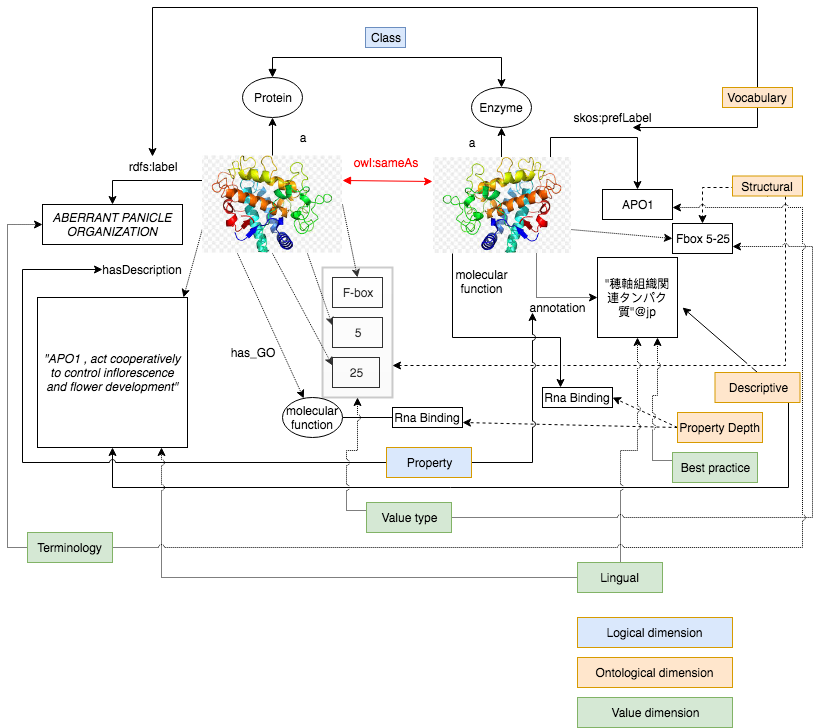
\includegraphics[width=1\textwidth]{Figures/exempleLiage.png}
\end{center}
\caption{\label{exempleL} Schéma général d'un exemple de liage de données inspiré de ~\cite{achichi2018} }
\end{figure}

L'état de l'art des méthodes ont été implémentés dans de nombreux logiciels dont les suivants sont les plus cités ou plus récents:


\begin{itemize}
%\item  \textbf{RDF-AI}~\cite{Scharffe2009} est un outil semi-automatique qui agit sur les trois étapes principales de la liaison de données. Il prend en entrée deux ensembles de données RDF et deux fichiers de configuration XML et génère en sortie un nouvel ensemble de données résultant de la fusion des deux ensembles de données en entrée ou une liste de correspondances entre des ressources équivalentes des deux ensembles de données. Le fichier de configuration XML spécifie les opérations de prétraitement à effectuer (vérification de la cohérence, traduction des propriétés, techniques de liaison, transformation des propriétés) pour chaque ressource. En effet, l'étape de pré-traitement génère deux données traitées par les opérations de l'utilisateur. Le deuxième fichier de configuration décrit les paramètres de post-traitement tels que le seuil de corrélation et les paramètres de fusion. Le système comprend deux algorithmes de calcul de similarité: un algorithme de correspondance de chaînes et un algorithme de relations de mots. Ce dernier a deux implémentations: un algorithme de comparaison de synonymes basé sur WordNet et un algorithme de similarité taxonomique basé sur le vocabulaire SKOS. Enfin, le système vérifie les incohérences (par exemple, la rupture des axiomes d'ontologies) qui peuvent apparaître à la suite du jeu de liens ou du graphe fusionné.

\item \textbf{Silk}~\cite{Jentzsch} met en œuvre des méthodes d'indexation et de présélection d'entités. La présélection consiste à rechercher un ensemble limité d’entités cibles susceptibles de correspondre à une entité source donnée. Toutes les ressources cibles sont indexées par une ou plusieurs valeurs de propriété spécifiée (le plus souvent, leurs labels). Le \textit{rdfs: label} d'une ressource source est utilisé comme terme de recherche dans les index générés et seules les premières ressources cibles trouvées dans chaque index sont considérées comme des liaisons possibles pour la correspondance. Cette stratégie ne garantit pas la découverte de toutes les ressources équivalentes dans le jeu de données cible. Silk est basé sur les règles de liage définies par l'utilisateur (Silk-LSL). En d'autres termes, il comporte un langage déclaratif permettant de spécifier les types de liens RDF à découvrir entre les sources de données et les conditions que doivent remplir les entités pour pouvoir être interconnectées.\\

\item \textbf{Limes}~\cite{Ngomo2011} se configure à l'aide d'un langage de spécification permettant d'identifier les liens. LIMES (comme Silk) propose de l'apprentissage supervisé  et de l'apprentissage actif pour la spécification des règles de liage. Pour cela, Silk et LIMES utilisent une programmation génétique. Cette dernière part d'un ensemble de spécifications de liens aléatoires et utilise les principes évolutifs de sélection et de variation pour faire évoluer ces spécifications jusqu'à ce qu'une condition de liaison réponde à un critère d'optimisation prédéfini (fonction fitness) ou qu'un nombre maximal d'itérations soit atteint. Pour l'apprentissage supervisé, des liens candidats validés manuellement sont utilisés dans l'algorithme génétique pour rechercher des liens similaires des règles de correspondance identifiées dans les données d'apprentissage. L’apprentissage actif vise à réduire la tache de labellisation des données d'entraînement en mettant en oeuvre un étiquetage interactif des candidats au liage selectionnés automatiquement. Dans ce cas, les liens candidats sont sélectionnés pour optimiser la similarité avec des instances non étiquetées. Par ce moyen, LIMES partitionne l'espace métrique (d'instance) en représentant chacune de ces parties au moyen d'un exemple permettant de calculer une approximation précise de la distance entre instances sur la base de distances déjà connues. Grâce au gain considérable d’efficacité apporté par l’outil, LIMES est capable de relier de très grands ensembles de données, là où d’autres outils échouent.\\


\item \textbf{Legato}~\cite{AchichiBT17} est conçu pour lier les entités de graphes ayant un haut degré d'hétérogénéité, se caractérisant par un faible recouvrement de ces ressources. L'outil est composé de module qui s'enchaine dans un workflow pour effectuer les différentes étapes necessaires aux liage. Le module de nettoyage des données ne conserve que les propriétés comparables entre les jeux de données (par conséquent, les commentaires sous forme de texte libre, ainsi que les identifiant d'instances spécifiques à une ressources sont supprimés). Le module de profilage d'instance représente les instances par un sous-graphe correspondant à l'union du CBD (Concise Bouded Description) de chaque ressource et de ses voisins directs. En cela, contrairement à SILK ou Limes, Legato (dans sa version par défaut) ne compare pas les valeurs de propriétés, mais considère toutes les valeurs littérales extractibles comme un sac de mots. Cette représentation aborde dans son mécanisme un certain nombre d'hétérogénéités de données sans nécessiter l'intervention de l'utilisateur, en particulier les différences de description et les différences de profondeur de propriété décrites ci-dessus. Les littéraux de ces sous-graphes sont ensuite utilisés pour projeter chaque instance dans un espace vectoriel et la mise en correspondance consiste à comparer les vecteurs résultants. Un seuil délibérément bas est utilisé pour la similarité vectorielle afin d'assurer un rappel élevé. Ensuite, des instances très similaires sont regroupées à l'aide d'un algorithme de classification hiérarchique standard. Un algorithme découverte de clé RDF~\cite{SymeonidouAPS1417} et un algorithme de classement de clé~\cite{Achichi2016} sont appliqués sur chaque paire de cluster similaires sur les deux graphes, afin d'identifier le jeu de propriétés qui permet le mieux de discriminer les ressources contenues dans chaque cluster. Un nouveau jeu de liens (appelé "liens sûrs") résulte de ce processus et est ensuite comparé aux liens produits à l'étape de mise en correspondance (appelés "liens candidats") afin d'éliminer les erreurs et d'augmenter la précision, aboutissant à la production du jeu de liens final. Le résultat de Legato est présenté au format EDOAL\footnote{\url{http://alignapi.gforge.inria.fr/edoal.html}}, ce qui permet de garder une trace des indices de confiance associés, ou sous forme de triplet \textit{owl:sameAs}. \\
\end{itemize}

Le liage de données est un composant très important dans le processus d’intégration de données car il permet d’agréger plusieurs propriétés/annotations autour d’une même entité enrichissant donc ses informations. Peu de méthodes ont été développées sur des données réelles et aucune dans le domaine agronomique. En collaboration avec Konstantin Todorov (MdC, Lirmm) nous proposerons d'évaluer les outils issus de l'état de l'art cités précédemment et proposerons une méthode adaptée au contexte d’AgroLD. \\


Nous proposons trois directions de recherche - éventuellement combinées - pour résoudre ce problème:
\begin{itemize}

\item \textbf{Extraction de données non structurées}: les graphes RDF contiennent du contenu textuel riche tel que des labels, des commentaires ou des descriptions qui fournissent une bonne information contextuelle. Ces contenus contiennent des entités et des relations susceptibles de compléter l'information nécessaire à la création de liens entre les jeux de données non-liés. Nous exploiterons ce contenu textuel en utilisant des techniques de traitement du langage naturel et d'extraction de relations pour identifier les entités nommées et reconstruire leurs relations, permettant ainsi la découverte de liens pertinents entre des ressources connexes.

 \item Les \textbf{techniques d'augmentation de graphe de connaissances} ajoutent des informations structurées aux graphes RDF existants en explorant des données externes pertinentes sur le Web (e.g. données de balisage, articles scientifiques, médias (sociaux), autres graphes de connaissances). Ce processus est particulièrement efficace pour récupérer des relations manquantes entre entités déjà présentes dans un graphe de connaissances. Nous appliquerons ces méthodes pour augmenter nos jeux de données en entrée et reconstruire les informations manquantes.
 
\item \textbf{Apprentissage automatique pour des jeux de données complémentaires}. Nous allons explorer les critères pertinents qui représentent de manières effectives les ressurces inter-graphes et nous les classerons comme identiques (ou non) par apprentissage automatique. Nous utiliserons des  modèles vectoriels pour des paires d'instances et ferons de l'apprentissage sur les relations entrée-sortie à partir des données d'apprentissage. Un jeu de données d'entraînement sur les données AgroLD est actuellement en construction.\\

\end{itemize}

Cette année un sujet de thèse sera proposée au concours de l’école doctorale de l’Université Montpellier. \\

%\subsubsection*{Exemple 1:} 
%ensembl:OS01G0675800\\
%\hspace{0.5cm} agrold:description \hspace{0.2cm}	\``NAC transcription factor 14; OS01G0675800 protein; OsNAC protein like.\''\\
%
%oryzabase:11464\\
%\hspace{0.5cm}	Agrold:has\_identifier \hspace{0.2cm} rapdb:OS01G0675800
\begin{figure}[!ht]
\begin{center}
	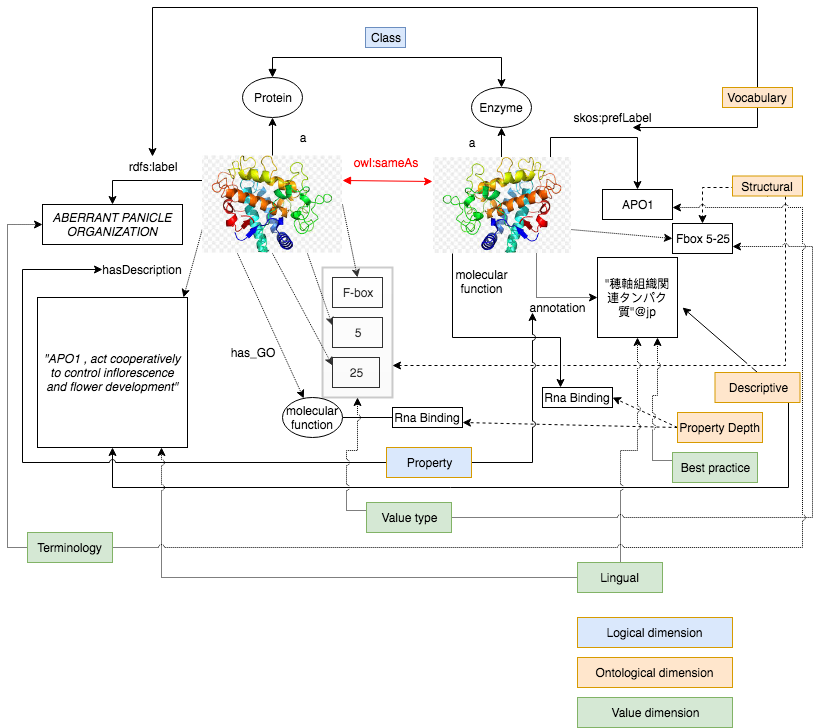
\includegraphics[width=1\textwidth]{Figures/exempleLiage.png}
\end{center}
\caption{\label{liage2} Exemple du problème de liage et d'interprétation automatique de champs textuel dans les données d’AgroLD}
\end{figure}


\subsection{Raisonnement sur les données}

Le fait que les données soient structurées en RDF présente l'avantage d'utiliser des mécanismes de requêtes tels que SPARQL pour exploiter au mieux les liens explicites existants entre les données (e.g. utilisation des propriétés is\_a dans les requêtes). Une autre manière d’enrichir ces liens est d’utiliser des mécanismes d’inférences qui grâce aux ontologies peuvent déduire de nouvelles connaissances implicites. Pour mener à bien cette problématique j’évaluerai les possibilités que proposent les langages SWRL, SPIN et SHACL  pour implémenter des règles d’enrichissement ou de vérification de cohérences dans les graphes.

\section{Applications sur les graphes de connaissances}
\subsection{Priorisation de gènes candidats}


Cette dernière phase du projet, intervient après l’intégration de nombreuses sources de données, la création et l’enrichissement de ces dernières sous forme de graphes de connaissance. La recherche d’information parmi ces graphes nécessite le développement de méthodes pour trier pertinemment les résultats.  La priorisation de gènes candidats permet d’identifier et de classer parmi un grand nombre de gènes, ceux qui sont fortement associés au phénotype ou la maladie étudiée. Il existe de nombreuses approches pour identifier des gènes candidats~\cite{Moreau2012}. \\

\subsubsection*{Méthodes basées sur des scores de co-occurrences}
La plus communément utilisée est l’approche « guilt by association » qui assume que les gènes associés ou interagissant dans un même processus partagent les mêmes fonctions. Les méthodes développées à partir de cette approche recherchent les mots clefs parmi un petit groupe de gènes annotés manuellement. La liste de gènes ainsi identifiés constitue une graine « seed genes » qui est ensuite utilisée pour trouver des associations avec les gènes à prioriser. 
Plus récemment, les approches de classement « ranking » ont émergé. Elles peuvent être divisée en 3 catégories : \\

\begin{enumerate}
\item Utilisant la fouille de données, 
\item Similarités de profil d’occurrences sur des sources multiples, 
\item Analyse topologique du réseau d’interaction moléculaire. \\
\end{enumerate}

Les applications Beegle~\cite{ElShal2016,Tranchevent2016a} et KnetMiner~\cite{Hassani-Pak2017a} sont de bon exemples à étudier car elles combinent les approches text mining (co-occurrence de termes) et intégration de sources multiples (TD/IDF, Algorithmes de ranking). Je compte approfondir ces aspects afin de proposer une méthode qui inclurai i) le calcul de scores pour chaque co-occurrence gène-phénotype trouvé dans une source (i.e. une source = un graphe), ii) la combinaison des différents résultats trouvé pour chaque source en pondérant les scores en fonction de l’origine des sources (i.e. source annotée manuellement, publication, etc.). Je continuerai à enrichir AgroLD en nouvelles connaissances et implémenter ces nouvelles méthodes dans l’interface de recherche. 

\subsubsection*{Méthodes basées sur l’analyse topologique du graphe de connaissance}

Récemment, certaines méthodes de ranking ont utilisé la topologie du réseau d’interaction gène-phénotype pour pondérer les scores de co-occurrences. Ces méthodes regardent si l’occurrence existe dans le voisinage du gène et calcule un score de distance en pondérant ce dernier en fonction de la nature des arrêtes et nœuds qui constitue ce chemin identifié. je compte aborder ces aspects, notamment par la méthode « Random Walk » en collaboration avec une équipe Vietnamienne qui travaillent sur ces methodes~\cite{Le2012,Le2013}

\subsection{Analyse fonctionnelle des réseaux d'interaction moléculaires}
Les graphes sont des outils très utiles et puissants pour représenter les interactions entre toutes les entités. Ainsi, ils sont parfaits pour représenter chaque type d'interactions qui se produisent dans les réseaux biologiques. Parcequ' RDF est un modèle de représentation basé sur un modèle multi-graphe orienté étiqueté, AgroLD contiendra plusieurs graphes representant la connaissance par domaine. Par exemple, les signaux de transduction dans les voix métaboliques, les réseaux de régulation de gènes ou les réseaux d'interaction proteine-proteine. Toutefois, il existe peu d'outils et d'algorithmes capables de gérer la visualisation et l'analyse d'énormes réseaux. \\
Comme point de départ, la topologie globale d'un réseau d'interaction, c'est-à-dire l'étude de propriétés principales telles que le coefficient de regroupement (clustering) ou le diamètre, peut révéler les principales propriétés du réseau. En plus de l'analyse des propriétés globales, l'étude de motifs topologiques locaux fréquents et l'extraction de modules pertinents (e.g. modules fonctionnels liés à la gene ontology) peuvent extraire des connaissances pertinentes. Enfin, la comparaison des sous-réseaux renforce les capacités de recherche en permettant par exemple la comparaison de réseaux correspondant à différents états (par exemple sains ou malades).

\section{Conclusion}
A travers ce projet de recherche, nous avons essayé de décrire le développement de méthodes permettant de gérer et structurer la complexité des données biologiques afin d'en extraire de la connaissance. Cette connaissance enrichie ayant pour objectif d’identifier les mécanismes moléculaires contrôlant l’expression de phénotypes chez les plantes. La finalité de ce projet même s'il est de nature pluri-disciplinaire reste avant tout tourné vers la biologie. L’objectif de ce projet sera en effet, de développer des approches de priorisation de gènes candidats utilisant un réseau d’interaction moléculaires comprenant des sources multiples issues de graphes de connaissances. Les méthodes de priorisation actuelles n'utilisent que que rarement ce type d'approche et elles restent encore moins avancées dans le domaine agronomique. 

Dans le domaine informatique, nous proposons plusieurs axes de travail tous participant un objectif commun: l'extraction et la publication de connaissances sur le web de données. Les méthodes que nous souhaitons développé s'appuient sur des données réelles ou des plateformes de production de données. Elles identifient donc des besoins réels et auront un impact important pour les communautés qui les utilisent.

Les résultats de ce projet seront importants pour les scientifiques de l’unité Diade mais également des collaborateurs, car il existe actuellement un réel verrou dans la gestion et le traitement des données biologiques. Ce projet revêt également un aspect important de collaboration avec des centres internationaux comme l’IRRI (le centre international du riz basé aux Philippines) et l'AfricaRice dans le cadre du workpackage « Big Data integration platform » du projet international Rice CRP. Il trouve également une place dans l'initiative Européenne Elixir-Exelerate sur le développement d'une infrastructure Bioinformatique pour l'échange de données et de services sur le web.  



